\documentclass[12pt,twosides,onecolumn,openany]{article}
\usepackage{graphicx} 


\usepackage[catalan]{babel}
\usepackage{emptypage}
\usepackage{hyperref}
\usepackage{mathtools}
\usepackage{blindtext}
\usepackage{subfigure}
\usepackage[utf8]{inputenc}
\usepackage{caption}
\usepackage{subcaption}
\usepackage{wrapfig}
\usepackage[a4paper]{geometry}
\geometry{top=2.5cm, bottom=2.5cm, left=2.5cm, right=2.5cm}
\usepackage{fancyhdr}
\pagestyle{fancy}
\usepackage{amsmath}
\usepackage{amssymb}
\usepackage{amsfonts}
\providecommand{\norm}[1]{\lVert#1\rVert}
\hypersetup{colorlinks=true,urlcolor=blue,linkcolor=blue}
\usepackage{multirow}
\usepackage{multicol}
\usepackage{rotating}

\usepackage{titlesec}

\newenvironment{Figura}
  {\par\medskip\noindent\minipage{\linewidth}}
  {\endminipage\par\medskip}

\titleformat{\section}  % comando de sección a formatear
  {\fontsize{14}{16}\bfseries} % formato para toda la línea
  {\thesection} % cómo mostrar el número
  {0.4em} % espacio entre el número y el texto
  {} % formato solo para el texto
  [] % formato para después del texto


\fancyhf{}
\fancyhead[LO,RE]{Grup D3}
\fancyhead[RO,LE]{Pràctica Ia}
\fancyfoot[LO,RE]{\thepage}
\fancyfoot[RO,LE]{Laboratori de Termodinàmica - UAB}
\graphicspath{ {images/} }

\begin{document}

\begin{center}
    {\Large \textsc{Transport de la calor: Estudi del transport de la calor en una barra metàl·lica}}\\
    \vspace{0.2cm}
    \textsc{30 d'Octubre de 2024}\\
    \vspace{0.2cm}
    $\begin{matrix} 
    \text{Miguel A.} \hspace{1.5cm} & \text{Daniel B.} & \hspace{1.5cm} \text{Sergi R.}\\1637738 \hspace{1.5cm} & 1603508 & \hspace{1.5cm} 1607805
    \end{matrix}$
\end{center}
\begin{center}
    \textsc{\textit{RESUM}}
\end{center}
Lorem ipsum dolor sit amet, consectetur adipiscing elit, sed do eiusmod tempor incididunt ut labore et dolore magna aliqua. Ut enim ad minim veniam, quis nostrud exercitation ullamco laboris nisi ut aliquip ex ea commodo consequat. Duis aute irure dolor in reprehenderit in voluptate velit esse cillum dolore eu fugiat nulla pariatur. Excepteur sint occaecat cupidatat non proident, sunt in culpa qui officia deserunt mollit anim id est laborum. \cite{prueba}
\vspace{0.5cm}
\begin{multicols}{2}
\section{Introducció i objectius}
\begin{equation}\label{sol_estacionaria}
  \theta(x) = \theta_0e^{-px}
\end{equation}
\begin{multline}\label{sol_permanent}
  \theta(x,t) = \theta_0e^{-px} +\\
   + A_0e^{-mx}\cos{\left( \frac{2\pi}{\tau} -hx \right)} 
\end{multline}
\begin{equation}\label{prom_temp}
  \langle \theta(x,t) \rangle = \theta_0e^{-px}  
\end{equation}
\begin{equation}\label{desfasament}
  \varphi_i = hx_i
\end{equation}
\begin{equation}\label{increment_desfasament}
  \Delta \varphi_i = h\Delta x
\end{equation}
\begin{equation}\label{trobar_m}
  \frac{a_i}{a_j} = e^{-m(x_i-x_j)}
\end{equation}
\begin{equation}\label{valor_lambda}
  \lambda = \frac{1}{2}[Kr(m^2 - h^2)]
\end{equation}
\section{Resultats i discussió}
\subsection{Estat estacionari}
Segons el desenvolupament teòric que seguim no podem negligir les diferències de radi entre les tres barres metàl·liques. Mesurem a l'inici, al mig i al final el diàmetre de cada barra i obtenim els valors de la Taula \ref{Tau:diam_radis}.
\begin{Figura}
  \centering
  \captionof{table}{\footnotesize{Diametres i radis de cada metall}}
  \begin{tabular}{c|c}
    Material & $r$ ($\pm$0,001) [cm] \\
    \hline\hline
    Al & 1,524\\
    Cu-Zn & 1,518\\
    Fe & 1,573 
  \end{tabular}
  \label{Tau:diam_radis}
\end{Figura}
A més, al llarg de l'experiment el labortaori ha anat canviant lleugerament de temperatura ambient. Per aquest motiu a l'hora de calcular els increments de temperatura $\theta_x$ farem servir com a temperatura ambient de referència la mitjana de tres mesures (veure Taula \ref{T_ambient} a l'Annex). Per tant, el valor de la temperatura ambient al laboratori és: \(T_a = (24,73 \pm 0,40)\,\text{K}\).\\\\
A partir de les dades de temperatura obtingudes per a cada barra obtenim la gràfica de la Figura \ref{DeltaT_vs_d}. Es pot veure com l'increment de temperatura decau de forma exponencial amb la distància al punt calent, tal com es podia preveure del desenvolupament teòric (Equació \eqref{sol_estacionaria}). Fent servir codi en Python obtenim un ajust exponencial de les dades mesurades. Aquest ajust es pot observar també a la Figura \ref{DeltaT_vs_d}, i les dades dels coeficients ajustats a la Taula \ref{Tau:coef_exponencial}
\begin{Figura}
  \centering
  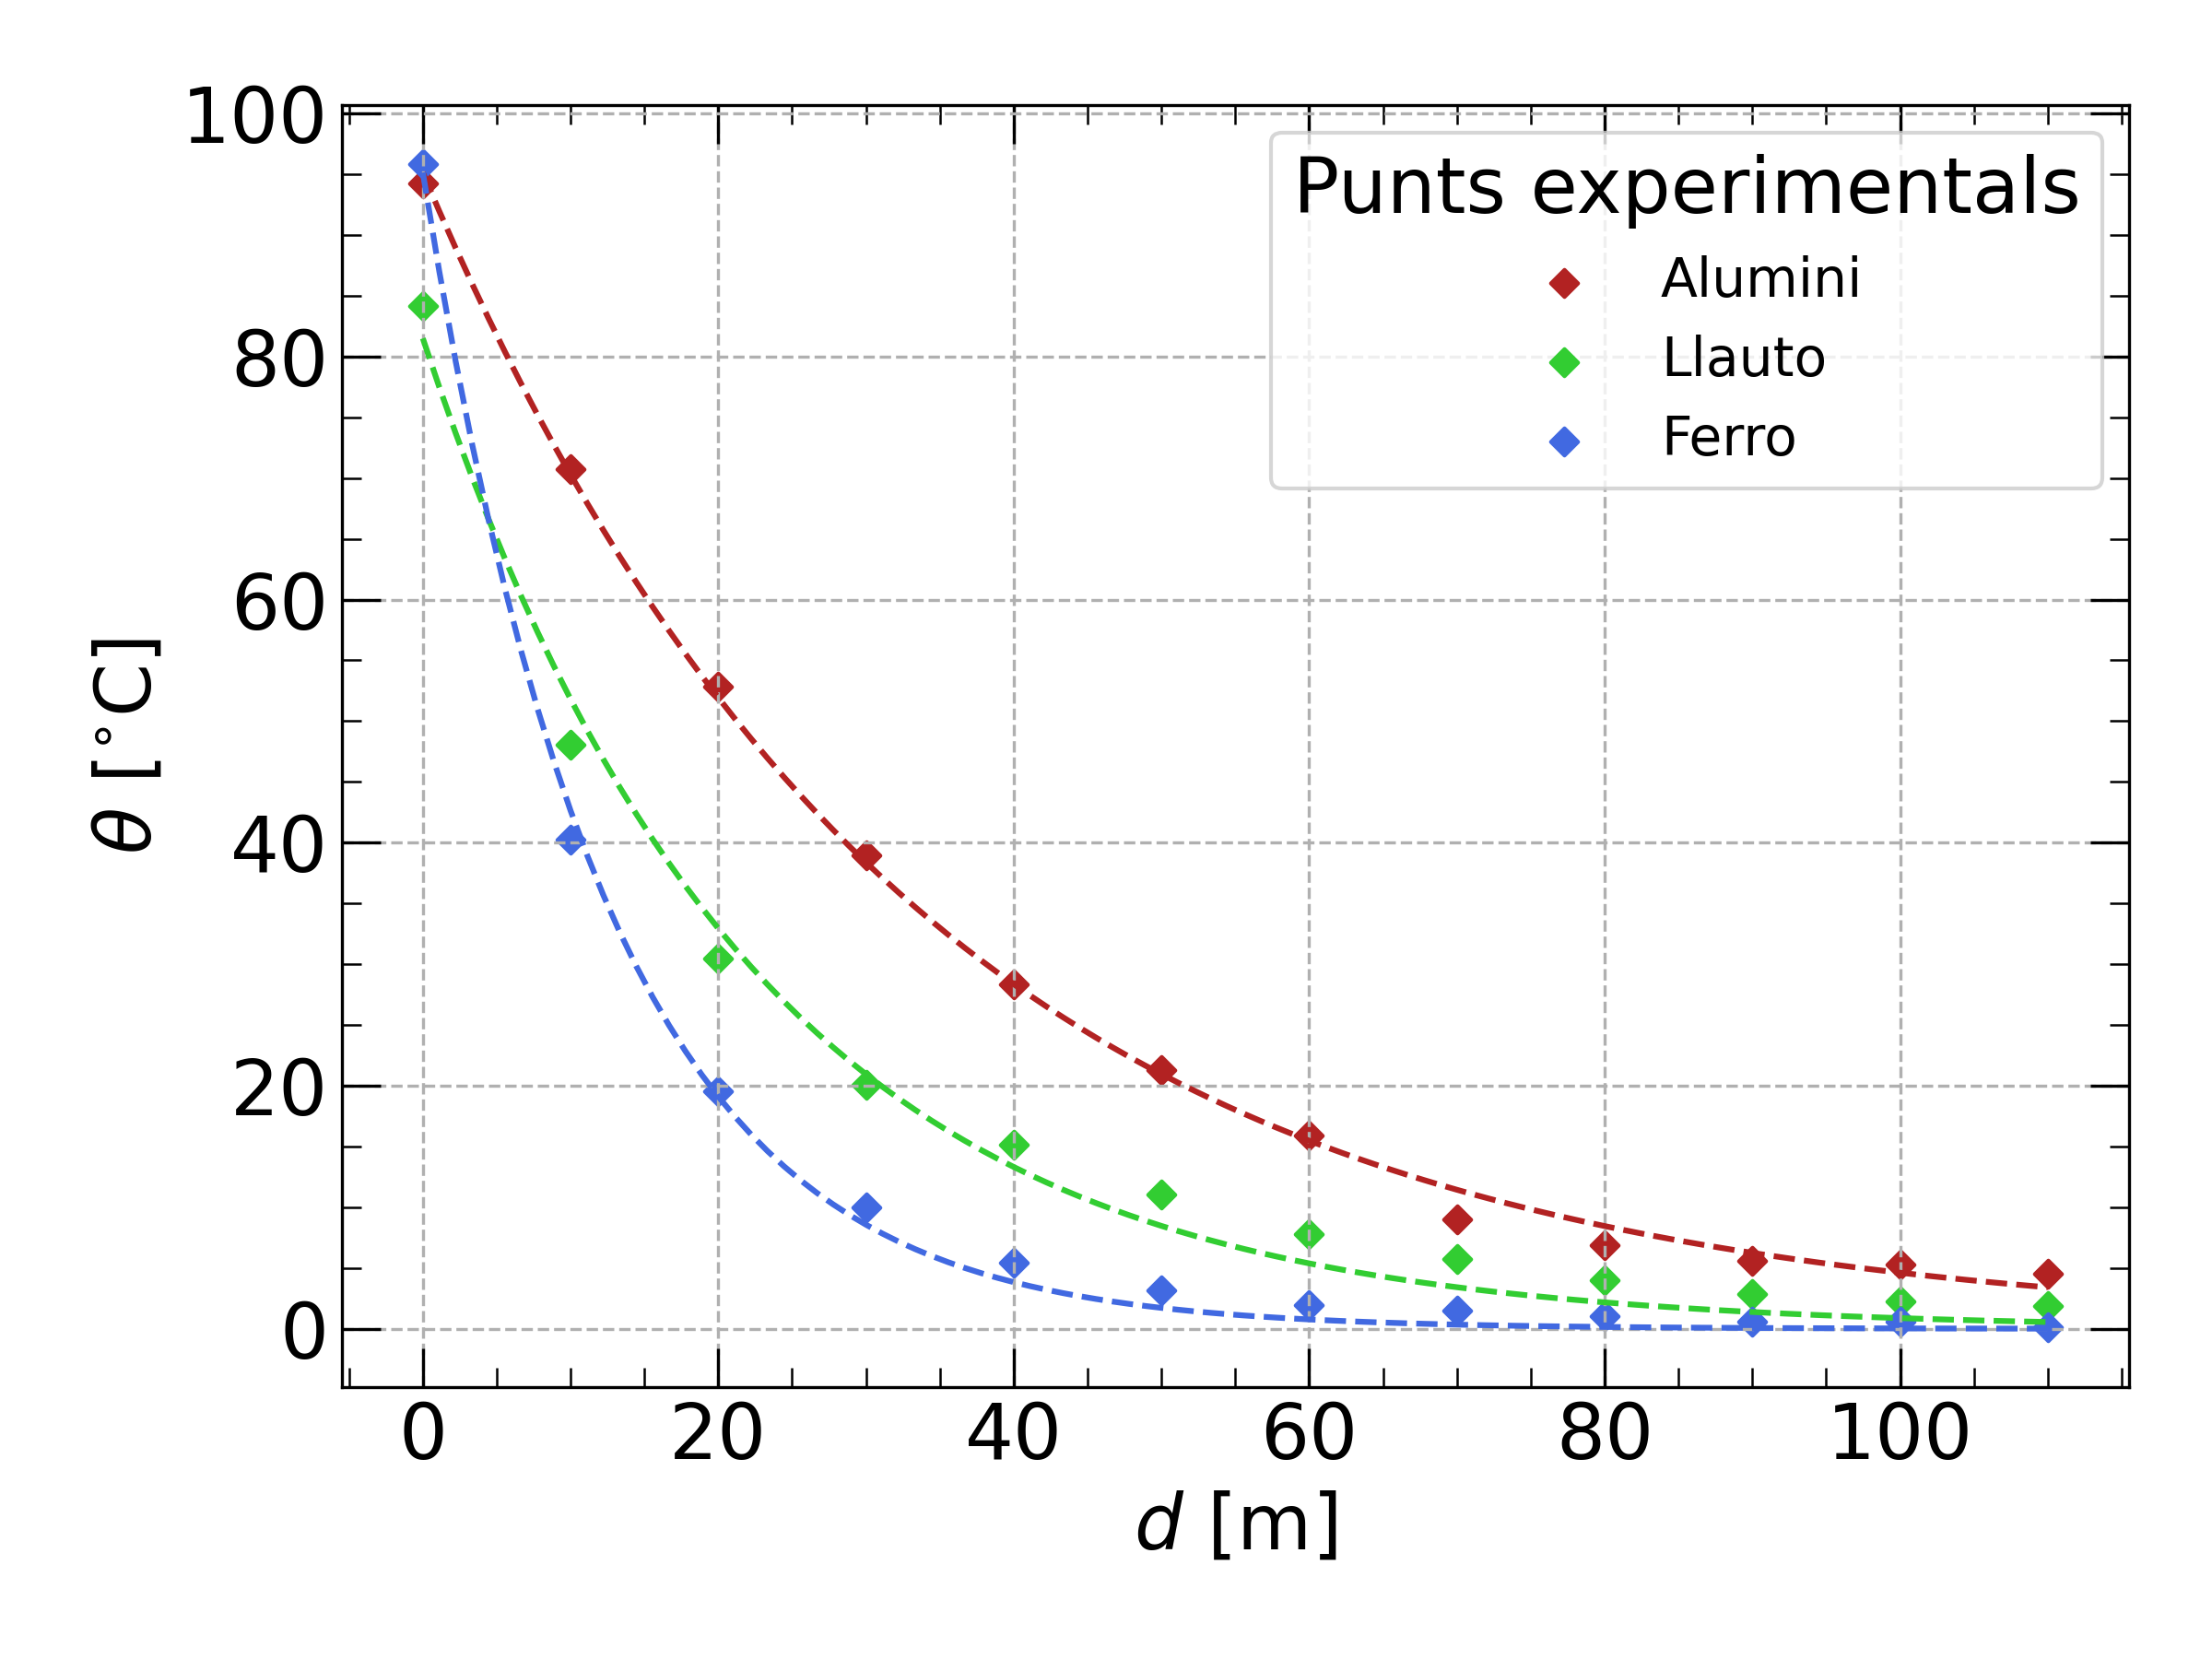
\includegraphics[width = 1\linewidth]{../../graphs/practica_Ia/plots/theta_vs_d_estacionaria.png}\label{DeltaT_vs_d}
  \captionof{figure}{\footnotesize{theta vs d}}
\end{Figura}

\begin{Figura}
  \centering
  \captionof{table}{\footnotesize{Coeficients $a$ i $b$ de l'ajust exponencial $y = ae^{bx}$ per als punts experimentals mesurats per l'alumini, el llautó i el ferro.}}
  \begin{tabular}{c|c|c}
    Material & $a$ [$^\circ$C] & $b$ ($\cdot 10^{-2}$) [cm$^{-1}$]\\
    \hline\hline
    Al & $95,11\pm0,97$ & $-3,025\pm0,051$\\
    Cu-Zn & $81,5\pm2,2$ & $-4,53\pm0,21$ \\
    Fe & $95,1\pm1,3$ & $-8,03\pm0,22$
  \end{tabular}
  \label{Tau:coef_exponencial}
\end{Figura}

Per a trobar el valor experimental de $p$ apliquem logaritme als valors experimentals per a poder realitzar una regressió lineal. Observem aquestes dades experimentals i les rectes de regressió a la Figura \ref{lnDeltaT_vs_d}. A la Taula \ref{Tau:dades_regressio} queden
\begin{Figura}
  \centering
  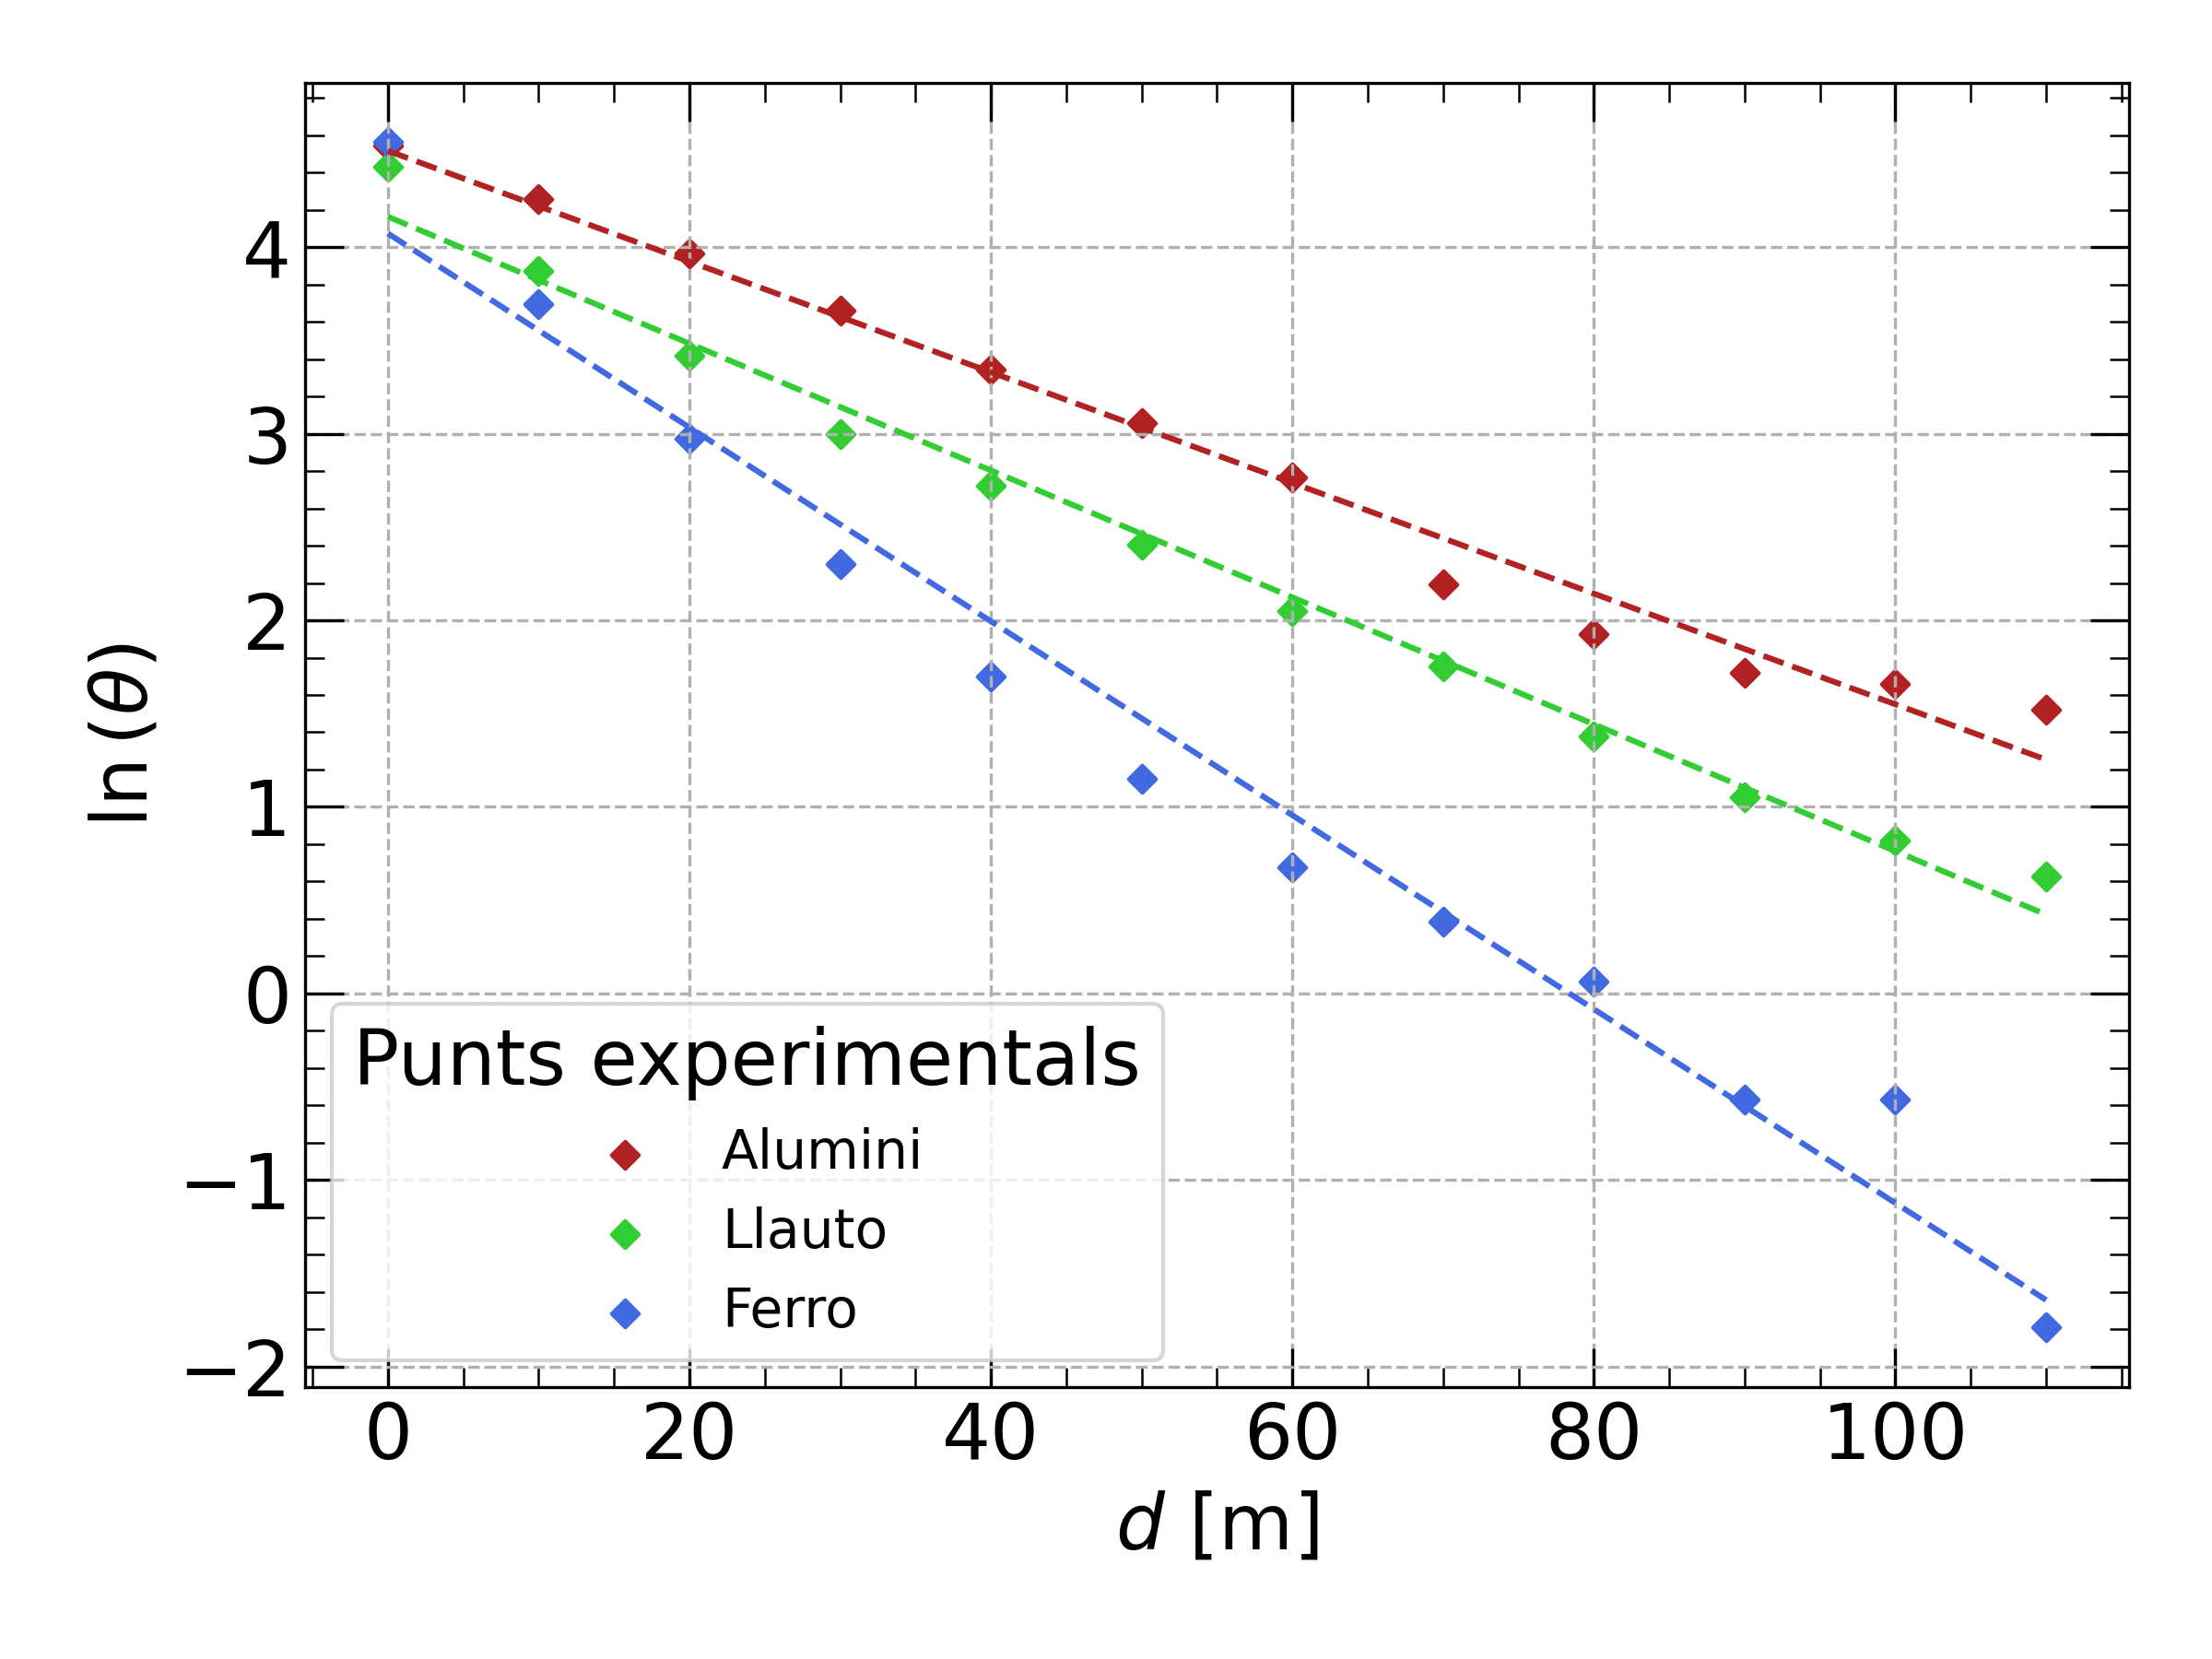
\includegraphics[width = 1\linewidth]{../../graphs/practica_Ia/plots/reg_estacionaria.png}\label{lnDeltaT_vs_d}
  \captionof{figure}{\footnotesize{Regressió lineal del logaritme de les temperatures per a cada material. Coeficients de regressió obtinguts: $r^2_{\text{Al}}=0.983$, $r^2_{\text{Cu-Zn}}=0.990$, $r^2_{\text{Fe}}=0.976$.}}
\end{Figura}           

\begin{Figura}
  \centering
  \captionof{table}{\footnotesize{Coeficients $a$ i $b$ de l'ajust lineal $y = ax + b$ per als punts experimentals mesurats per l'alumini, el llautó i el ferro.}}
  \begin{tabular}{c|c|c}
    Material & $a$ ($\cdot 10^{-2}$) [cm$^{-1}$] & $b$\\
    \hline\hline
    Al & $-2,97\pm0,12$ & $4,517\pm0,080$\\
    Cu-Zn & $-3,40\pm0,11$ & $4,164\pm0,070$ \\
    Fe & $-5,20\pm0,26$ & $4,07\pm0,17$
  \end{tabular}
  \label{Tau:dades_regressio}
\end{Figura}
Tenint en compte de l'equació \eqref{sol_estacionaria}, què val $p$ (valor absolut de les $a$ a la Taula \ref{Tau:dades_regressio}) i suposant el mateix valor constant del coeficient $\lambda$ per als tres metalls observem la temperatura d'un metall decau com $(Kr)^{1/2}$. Deduim doncs que la conductivitat tèrmica dels tres metalls és diferent i que es compleix
\begin{equation*}
  K_{\text{Fe}} < K_{\text{Cu-Zn}} < K_{\text{Al}} \hspace{3mm}
\end{equation*}
i que existeixen les relacions
\begin{equation*}
  \frac{K_ir_i}{K_jr_j} = \frac{p^2_j}{p^2_i}
\end{equation*}
on $i$ i $j$ prenen valors dels diferents metalls que estem estudiant. Fent recerca a la literatura trobem el valor de la conductivitat tèrmica del ferro: \(K_{\text{Fe}} =  0,802\, \text{V}/\text{cmK}\). Fent servir les relacions anteriors i el valor trobat a la literatura podem calcular, aproximadament, els valors de la conductivitat tèrmica dels altres dos metalls. Podem comparar aquests valors obtinguts amb els que podem trobar a la literatura. S'observen totes aquestes dades a la Taula \ref{Tau:conductivitats_termiques_Fe}.
\begin{Figura}
  \centering
  \captionof{table}{\footnotesize{Comparació de la conductivitat tèrmica experimental i teòrica segons el patró ferro.}}
  \begin{tabular}{c|c|c}
    Material & $K_{\text{exp}}$ [W/cmK] & $K_{\text{teo}}$ [W/cmK]\\
    \hline\hline
    Al & $2,54\pm0,25$ & 2,37\\
    Cu-Zn & $1,94\pm0,19$ & 1,09
  \end{tabular}
  \label{Tau:conductivitats_termiques_Fe}
\end{Figura}
Com a aproximació alternativa podem fer servir, en comptes del ferro, l'alumini com a patró. Aplicant les mateixes relacions que amb el ferro obtenim les dades de la Taula \ref{Tau:conductivitats_termiques_Al}.
\begin{Figura}
  \centering
  \captionof{table}{\footnotesize{Comparació conductivitats tèrmiques - Patró alumini}}
  \begin{tabular}{c|c|c}
    Material & $K_{\text{exp}}$ [W/cmK] & $K_{\text{teo}}$ [W/cmK]\\
    \hline\hline
    Cu-Zn & $1,81\pm0,15$ & 1,09\\
    Fe & $0,748\pm0,062$ & 0,802
  \end{tabular}
  \label{Tau:conductivitats_termiques_Al}
\end{Figura}
\textit{Explicaciones varias: explicar la discrepancia del patron aluminio, explicar que el latón da mucho error y puede que $\lambda$ no sea ni constante ni igual para todos, comentar que $K$ puede variar con la temperatura.}
\subsection{Estat permanent}
A partir de les dades obtingudes experimentalment representem l'evolució temporal de la temperatura segons cada posició de la barra gran, Figura \ref{fig:T_vs_t_gran}, i de la barra petita, \ref{fig:T_vs_t_petita}.
\begin{Figura}
  \centering
  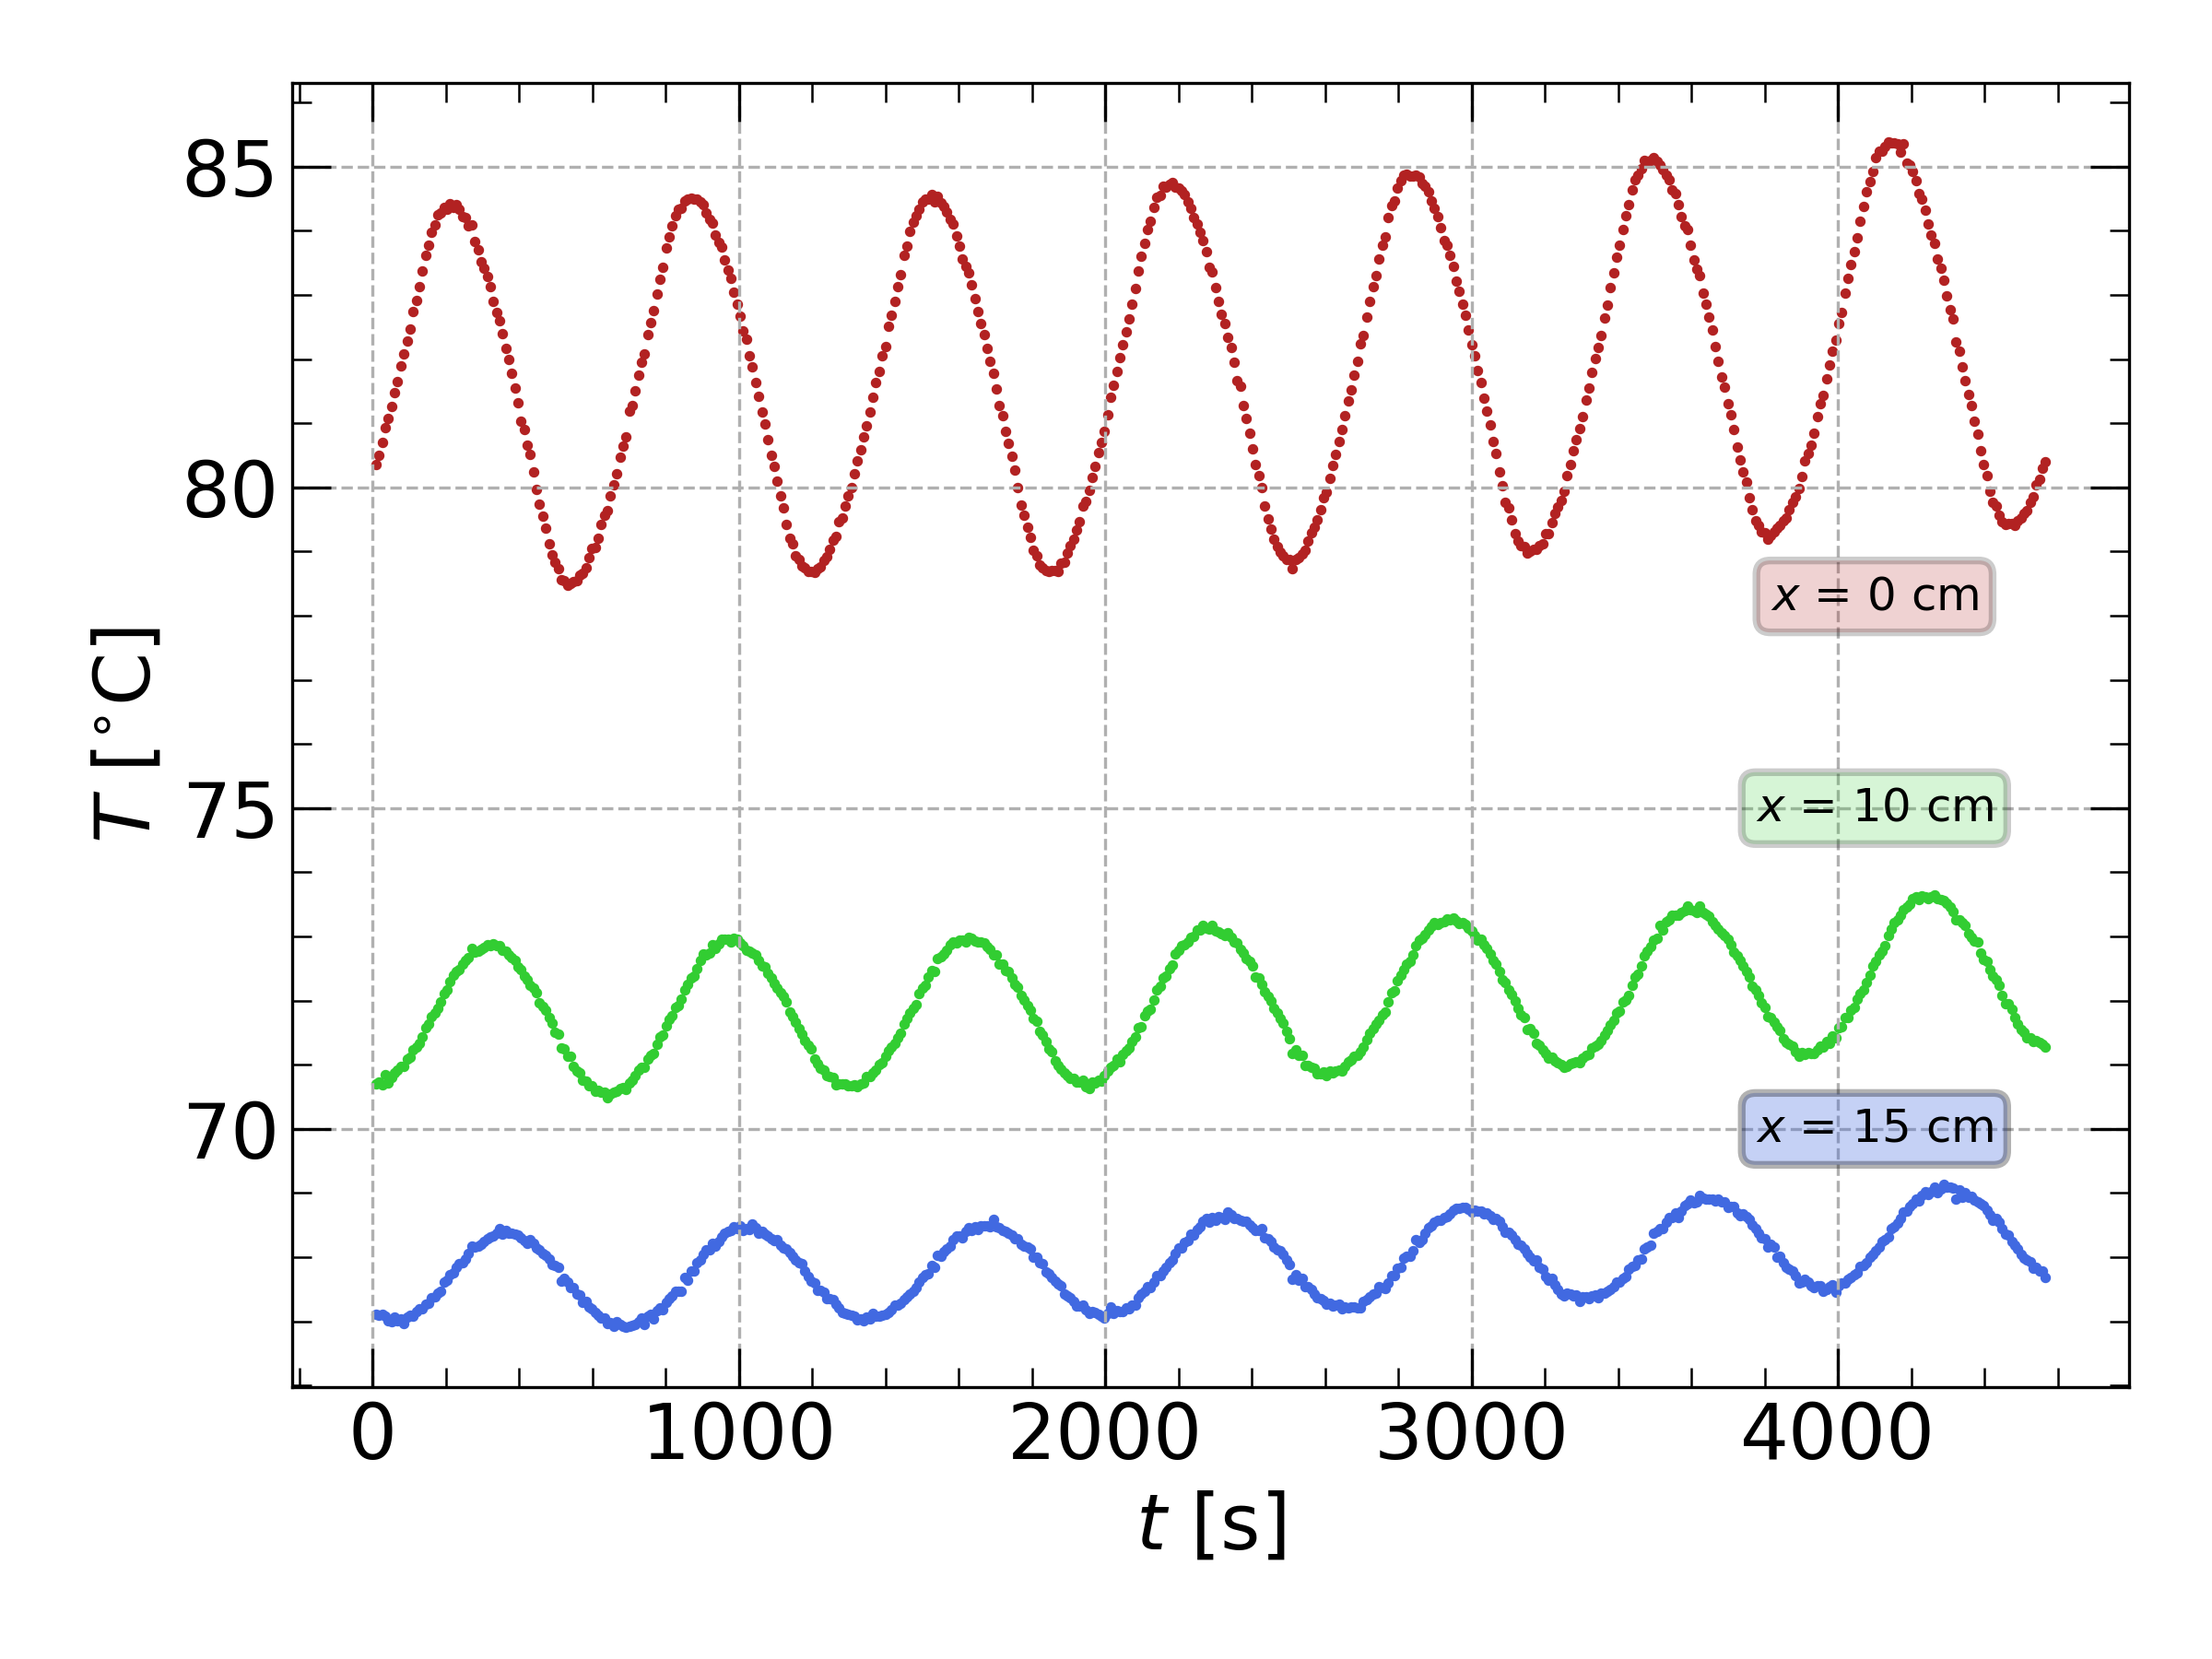
\includegraphics[width= 1\linewidth]{../../graphs/practica_Ia/plots/gran.png}
  \captionof{figure}{\footnotesize{Gràfica de $T$ en funció $t$ de la barra gran. Temperatures mesurades a una distància de \(0\,\text{cm}\) (vermell), \(10\,\text{cm}\) (verd) i \(15\,\text{cm}\) (blau) del punt de referència.}}
  \label{fig:T_vs_t_gran}
\end{Figura}
\begin{Figura}
  \centering
  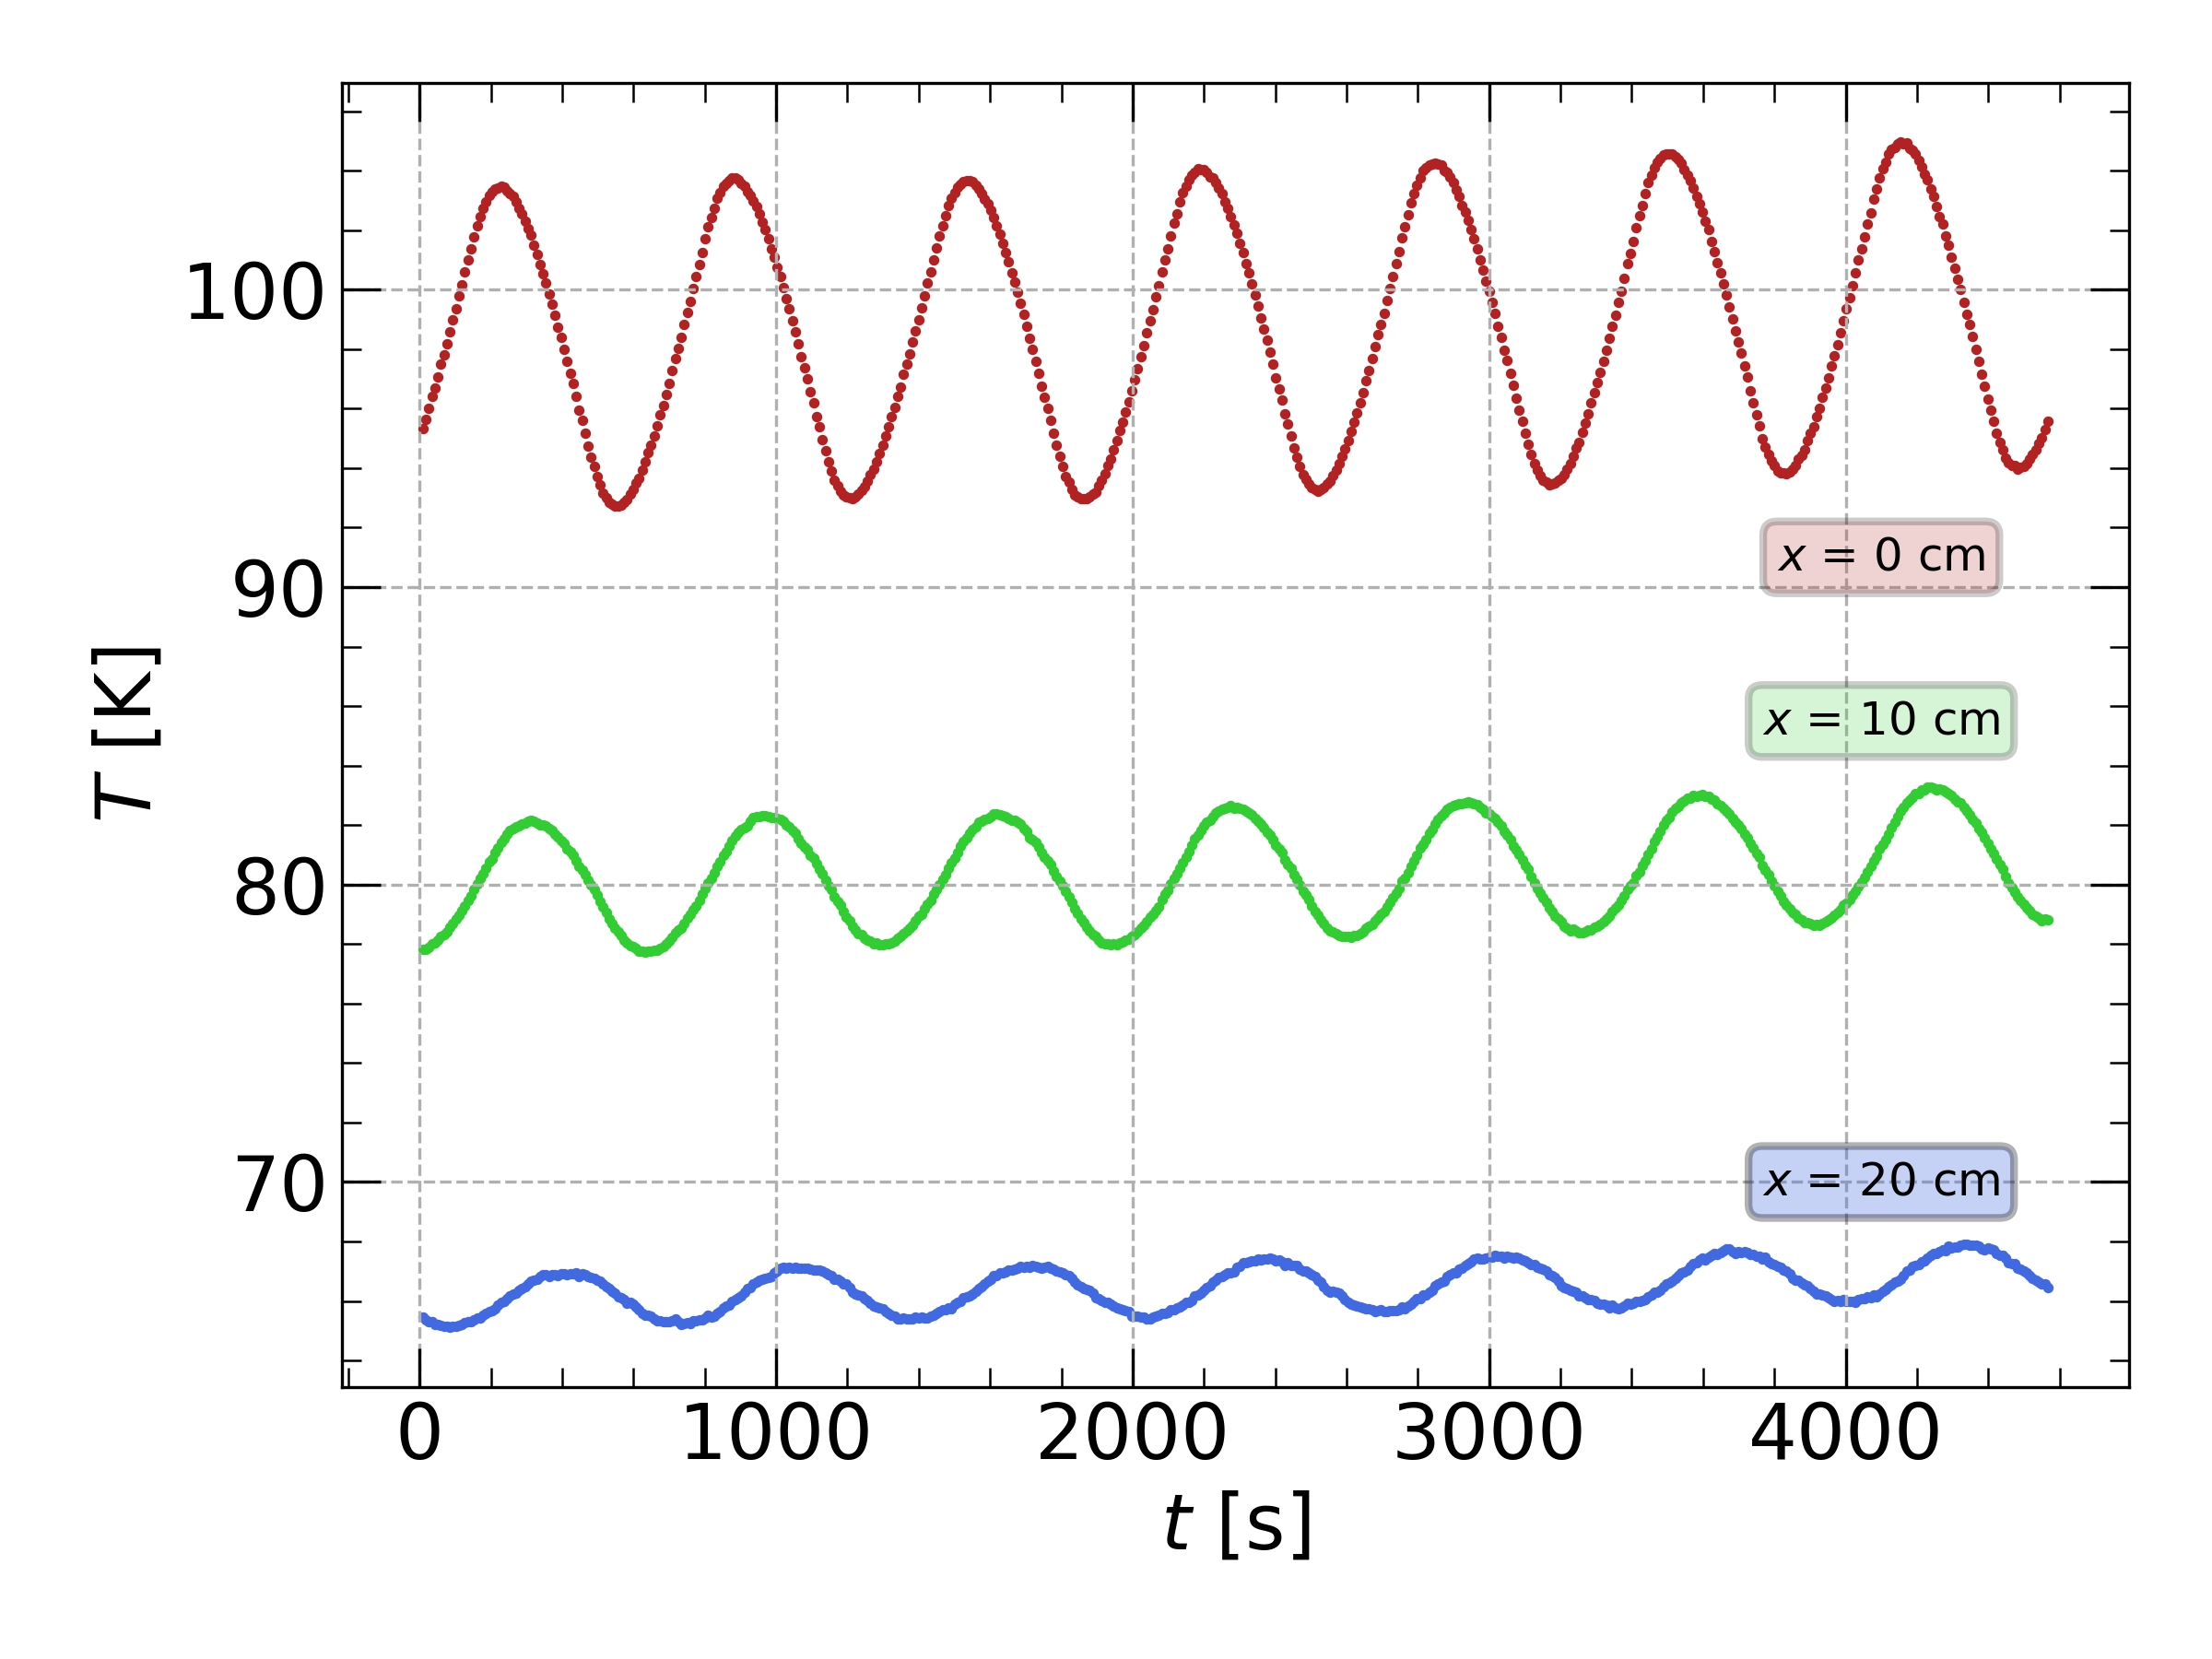
\includegraphics[width= 1\linewidth]{../../graphs/practica_Ia/plots/petita.png}
  \captionof{figure}{\footnotesize{Gràfica de $T$ en funció $t$ de la barra petita. Temperatures mesurades a una distància de \(0\,\text{cm}\) (vermell), \(10\,\text{cm}\) (verd) i \(20\,\text{cm}\) (blau) del punt de referència.}}
  \label{fig:T_vs_t_petita}
\end{Figura}
Notem com l'evolució temporal mesurada de la temperatura és coherent amb la solució de l'equació diferencial vista a l'Equació \eqref{sol_permanent}. El segón terme de la solució correspón a una funció periòdica en el temps que decau amb la distància i presenta un desfasament, també depenent de la distància. Tant a la Figura \ref{fig:T_vs_t_gran} com a la Figura \ref{fig:T_vs_t_petita} es veu que la temperatura és funció periòdica en el temps ( és una ona tèrmica) i que, quant més lluny del punt de referència ens trobem, més petita és l'amplitud de d'aquesta ona. Tot i ser complicat a simple vista veure-ho, existeix un desfasament entre les oscil·lacions de la mateixa barra a diferents distàncies. Per a observar millor aquest desfasament podem preparar les dades d'una forma més convenient.\\\\
Com a pas previ a observar el desfasament, calculem la temperatura mitjana a cada punt de cada barra. Com a simplificació, calculem aquesta mitjana temporal fent una mitjana aritmètica de les dades obtingudes al laboratori. Els valors d'aquestes mitjanes venen recollits a la Taula \ref{Tau:mitjanes}
\begin{Figura}
  \centering
  \captionof{table}{\footnotesize{Temperatura mitjana ($\langle \theta \rangle$) a cada posició $x_i$ per a la barra gran i la barra petita.}}
  \begin{tabular}{c|c}
    $x_i$ ($\pm$0,1) [cm] & $\langle \theta \rangle$ ($\pm$ 0,001) [$^\circ$C]\\
    \hline 
    \multicolumn{2}{c}{Barra gran} \\ \hline
    0 & 81,849\\
    10 & 72,012\\
    15 & 67,928 \\ \hline
    \multicolumn{2}{c}{Barra petita} \\ \hline
    0 & 98,717\\
    10 & 80,420\\
    20 & 66,486 \\
  \end{tabular}
  \label{Tau:mitjanes}
\end{Figura}
Observem com la temperatura mitjana decau amb la distància respecte a l'origen de referència. Clarament són pocs punts experimentals com per a traçar una corba de tendència. Tot i això, qualitativament els valors obtinguts s'apropen al que prediu la teoria. En cas de repetir l'experiment amb més termoparells repartits al llarg de cadascuna de les barres observariem un comportament de la mitjana temporal de la temperatura com el de l'Equació \eqref{prom_temp}. Si apliquem el mateix mètode que a l'estat estacionari per a obtenir el valor de $p$ obtenim els valors que s'observen a la Taula \ref{tau:pendent_mitjana}. A partir d'aquestes dades realitzem una regressió i observem, Figura \ref{fig:lin_reg} com s'apropen molt a un comportament lineal.
\begin{Figura}
  \centering
  \captionof{table}{\footnotesize{Valors ajustats per a una regressió lineal, amb model $y = ax + b$, on $y$ és el logaritme de les temperatures mitjanes i $x$ les posicions $x_i$.}}
  \begin{tabular}{c|c|c}
    Barra & $a$ ($\cdot 10^{-3}$) [cm$^{-1}$] & $b$ ($\cdot 10^{-2}$) \\ \hline\hline
    gran & $-12,43\pm0,29$ & $44,04\pm0,30$\\
    petita & $-19,75\pm0,42$ & $45,90\pm0,55$
  \end{tabular}
  \label{Tau:pendent_mitjana}
\end{Figura}
\begin{Figura}
  \centering
  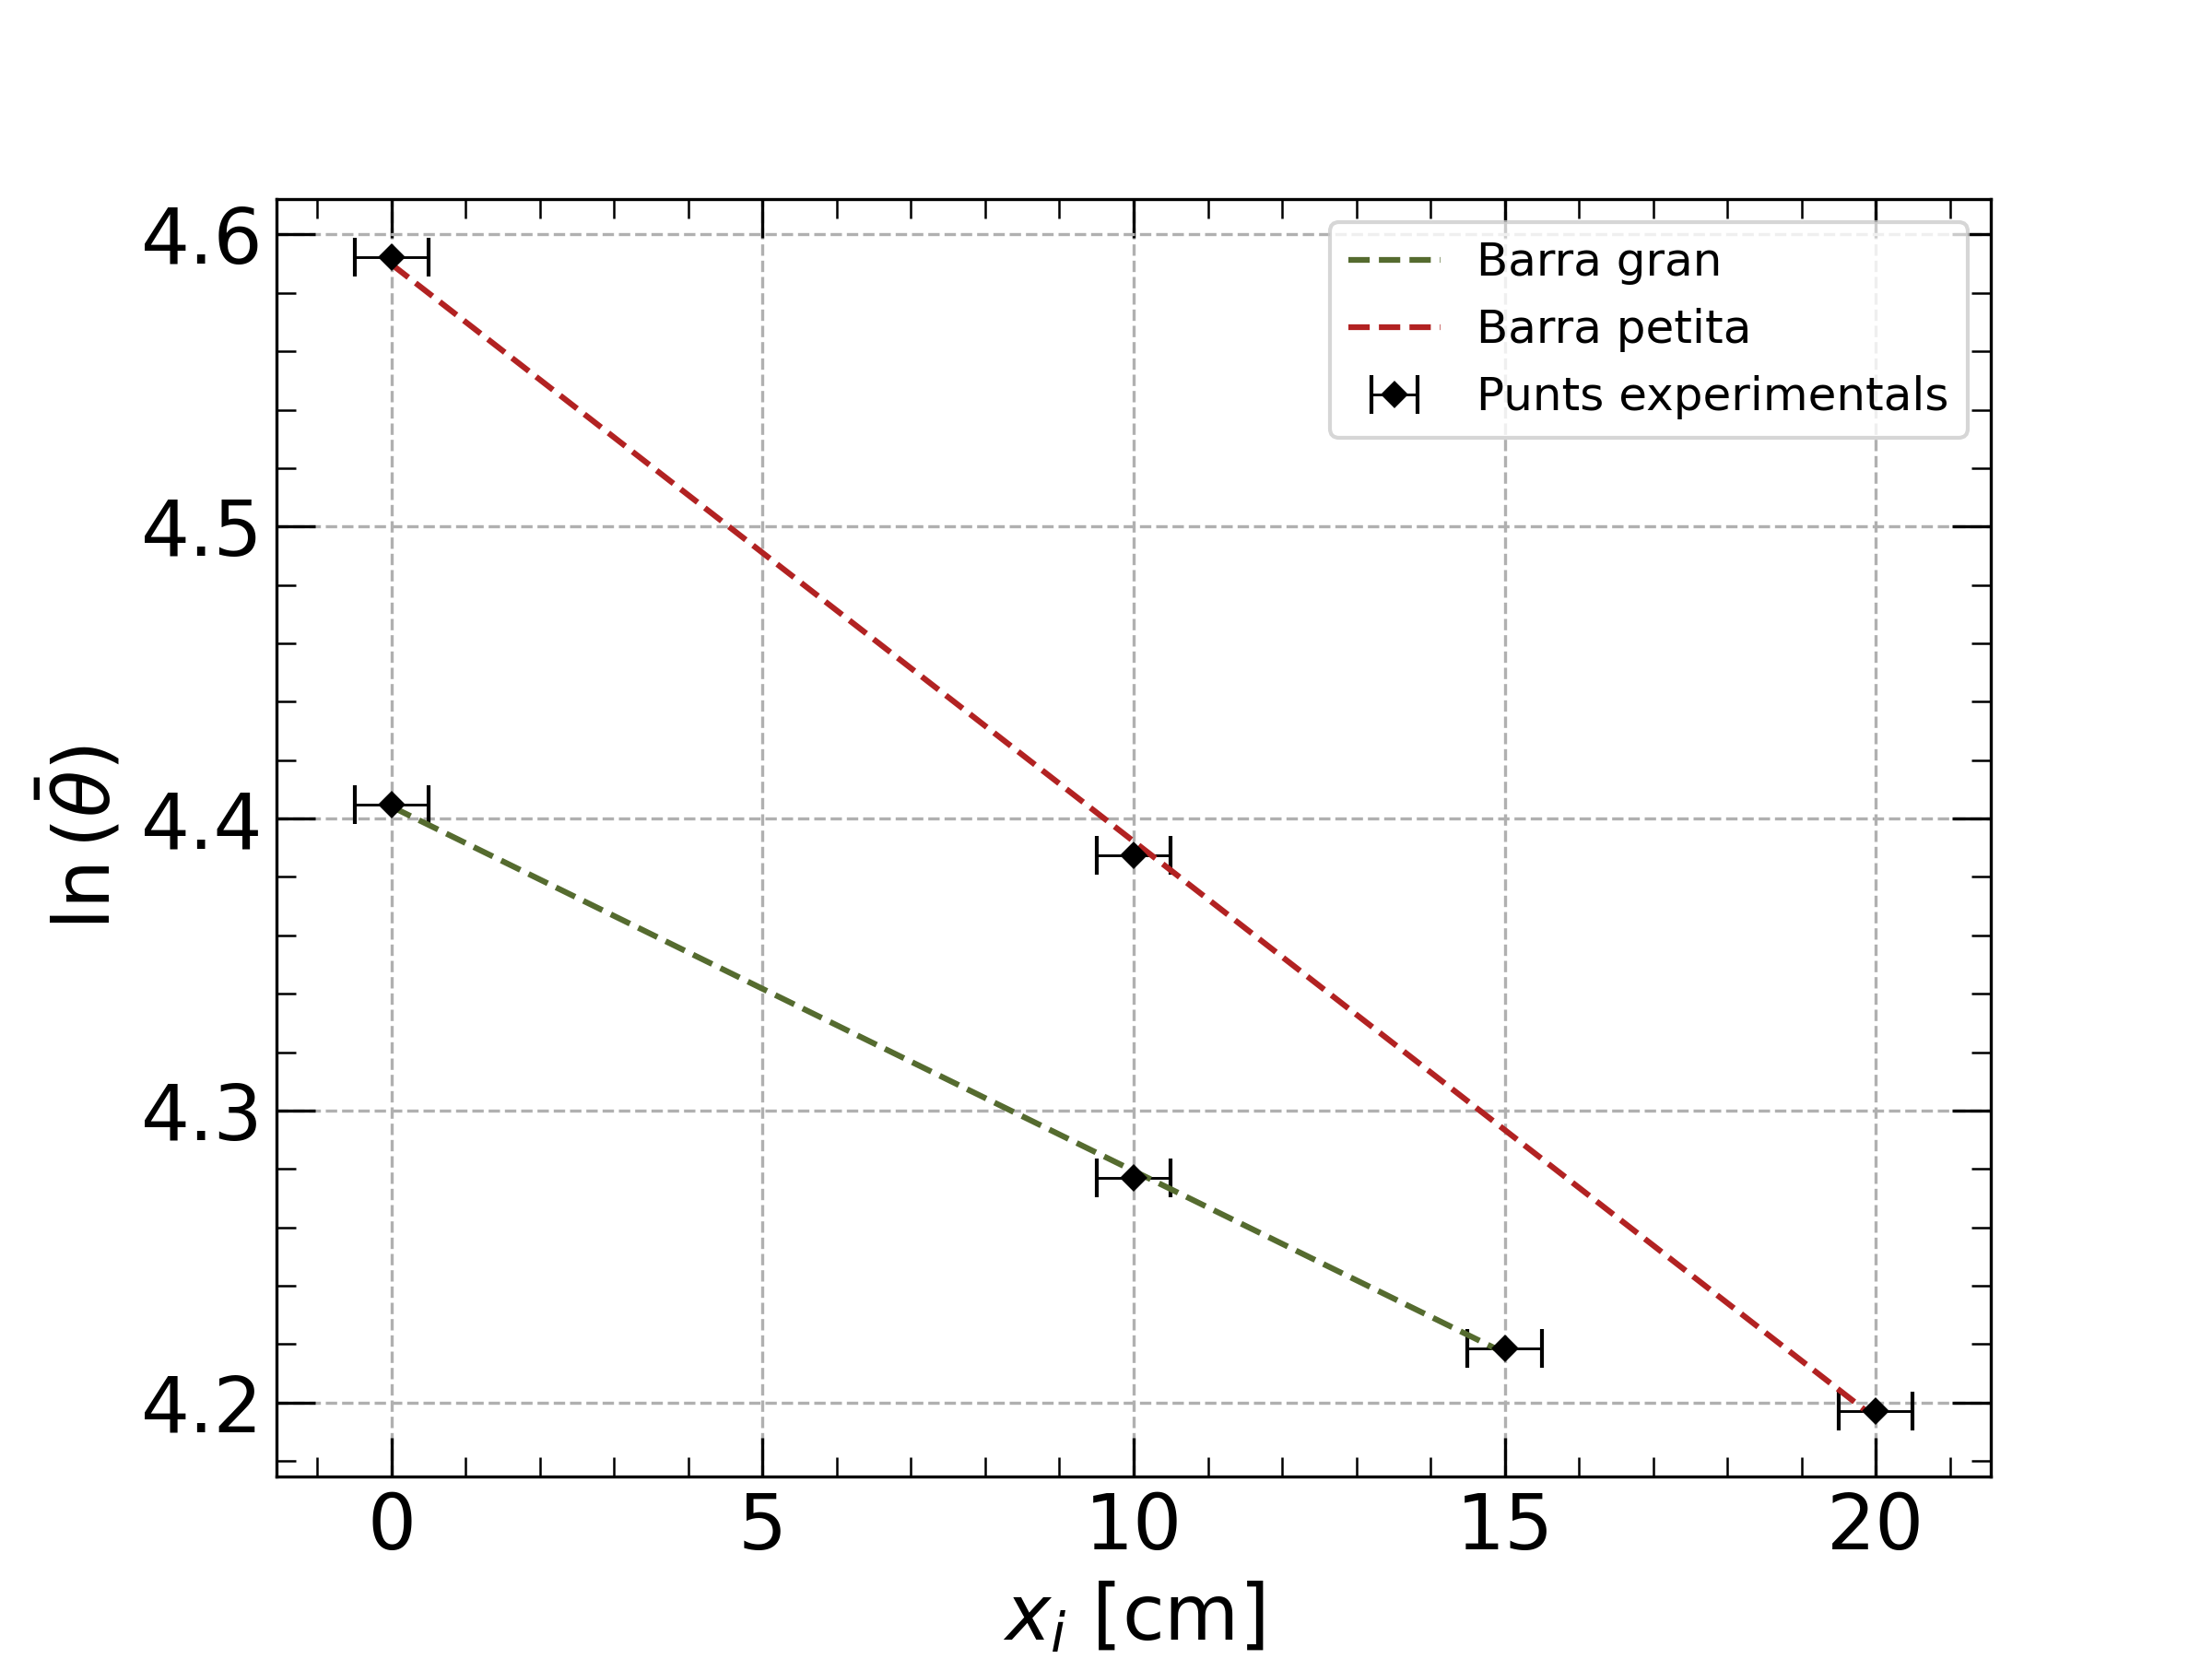
\includegraphics[width=1\linewidth]{../../graphs/practica_Ia/plots/linear_reg.png}
  \captionof{figure}{\footnotesize{Regressió lineal del logaritme de temperatures respecte a la posició. Coeficients de regressió obtinguts: $r^2$ = 0.999 tant per a la barra gran com per a la barra petita.}}
  \label{fig:lin_reg}
\end{Figura}
Un cop calculades les mitjanes per a cada punt, podem normalitzar les dades experimentals dividint per la seva temperatura mitjana corresponent. Aplicant aquest mètode i, per a obtenir més detall, escollint com a molt els dos primers periodes d'oscil·lació obtenim la Figura \ref{fig:T_vs_t_gran_norm} per a la barra gran i la Figura \ref{fig:T_vs_t_petita_norm} per a la barra petita.
\begin{Figura}
  \centering
  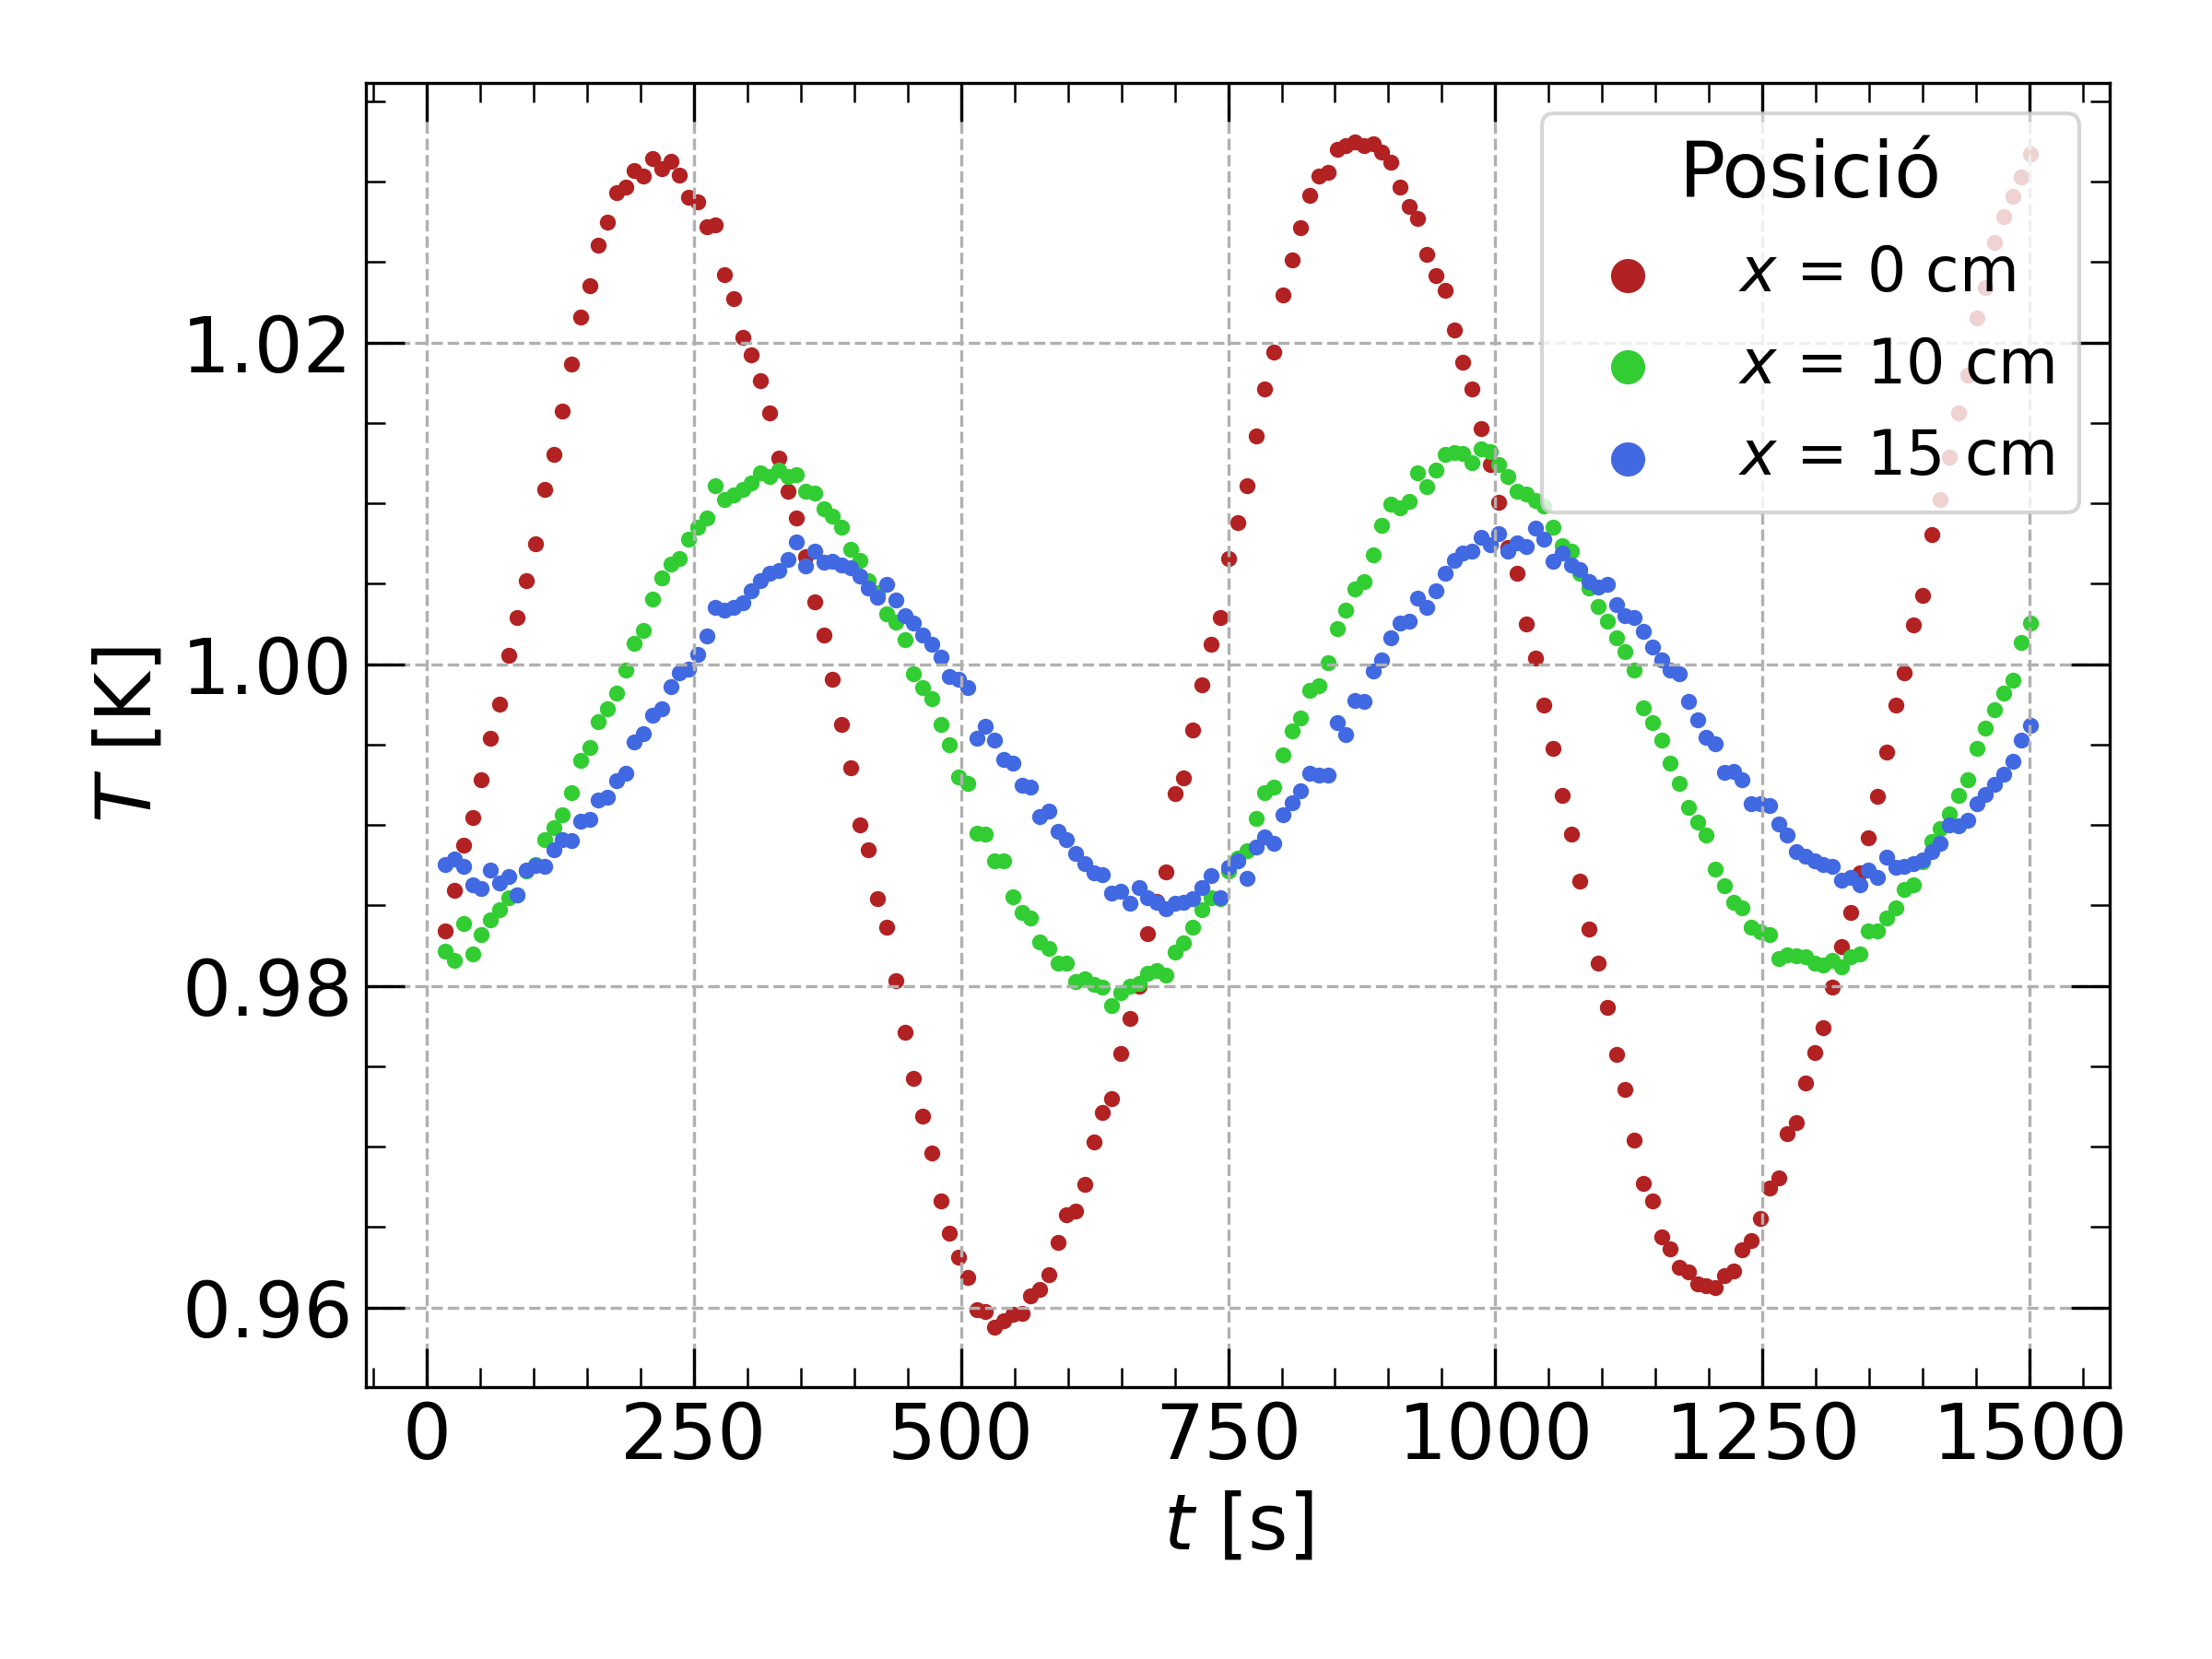
\includegraphics[width=1\linewidth]{../../graphs/practica_Ia/plots/gran_norm.png}
  \captionof{figure}{\footnotesize{Gràfica de $T$ en funció de $t$ normalitzada de la barra gran. Temperatures mesurades a una distància de \(0\,\text{cm}\) (vermell), \(10\,\text{cm}\) (verd) i \(15\,\text{cm}\) (blau) del punt de referència.}}
  \label{fig:T_vs_t_gran_norm}
\end{Figura}
\begin{Figura}
  \centering
  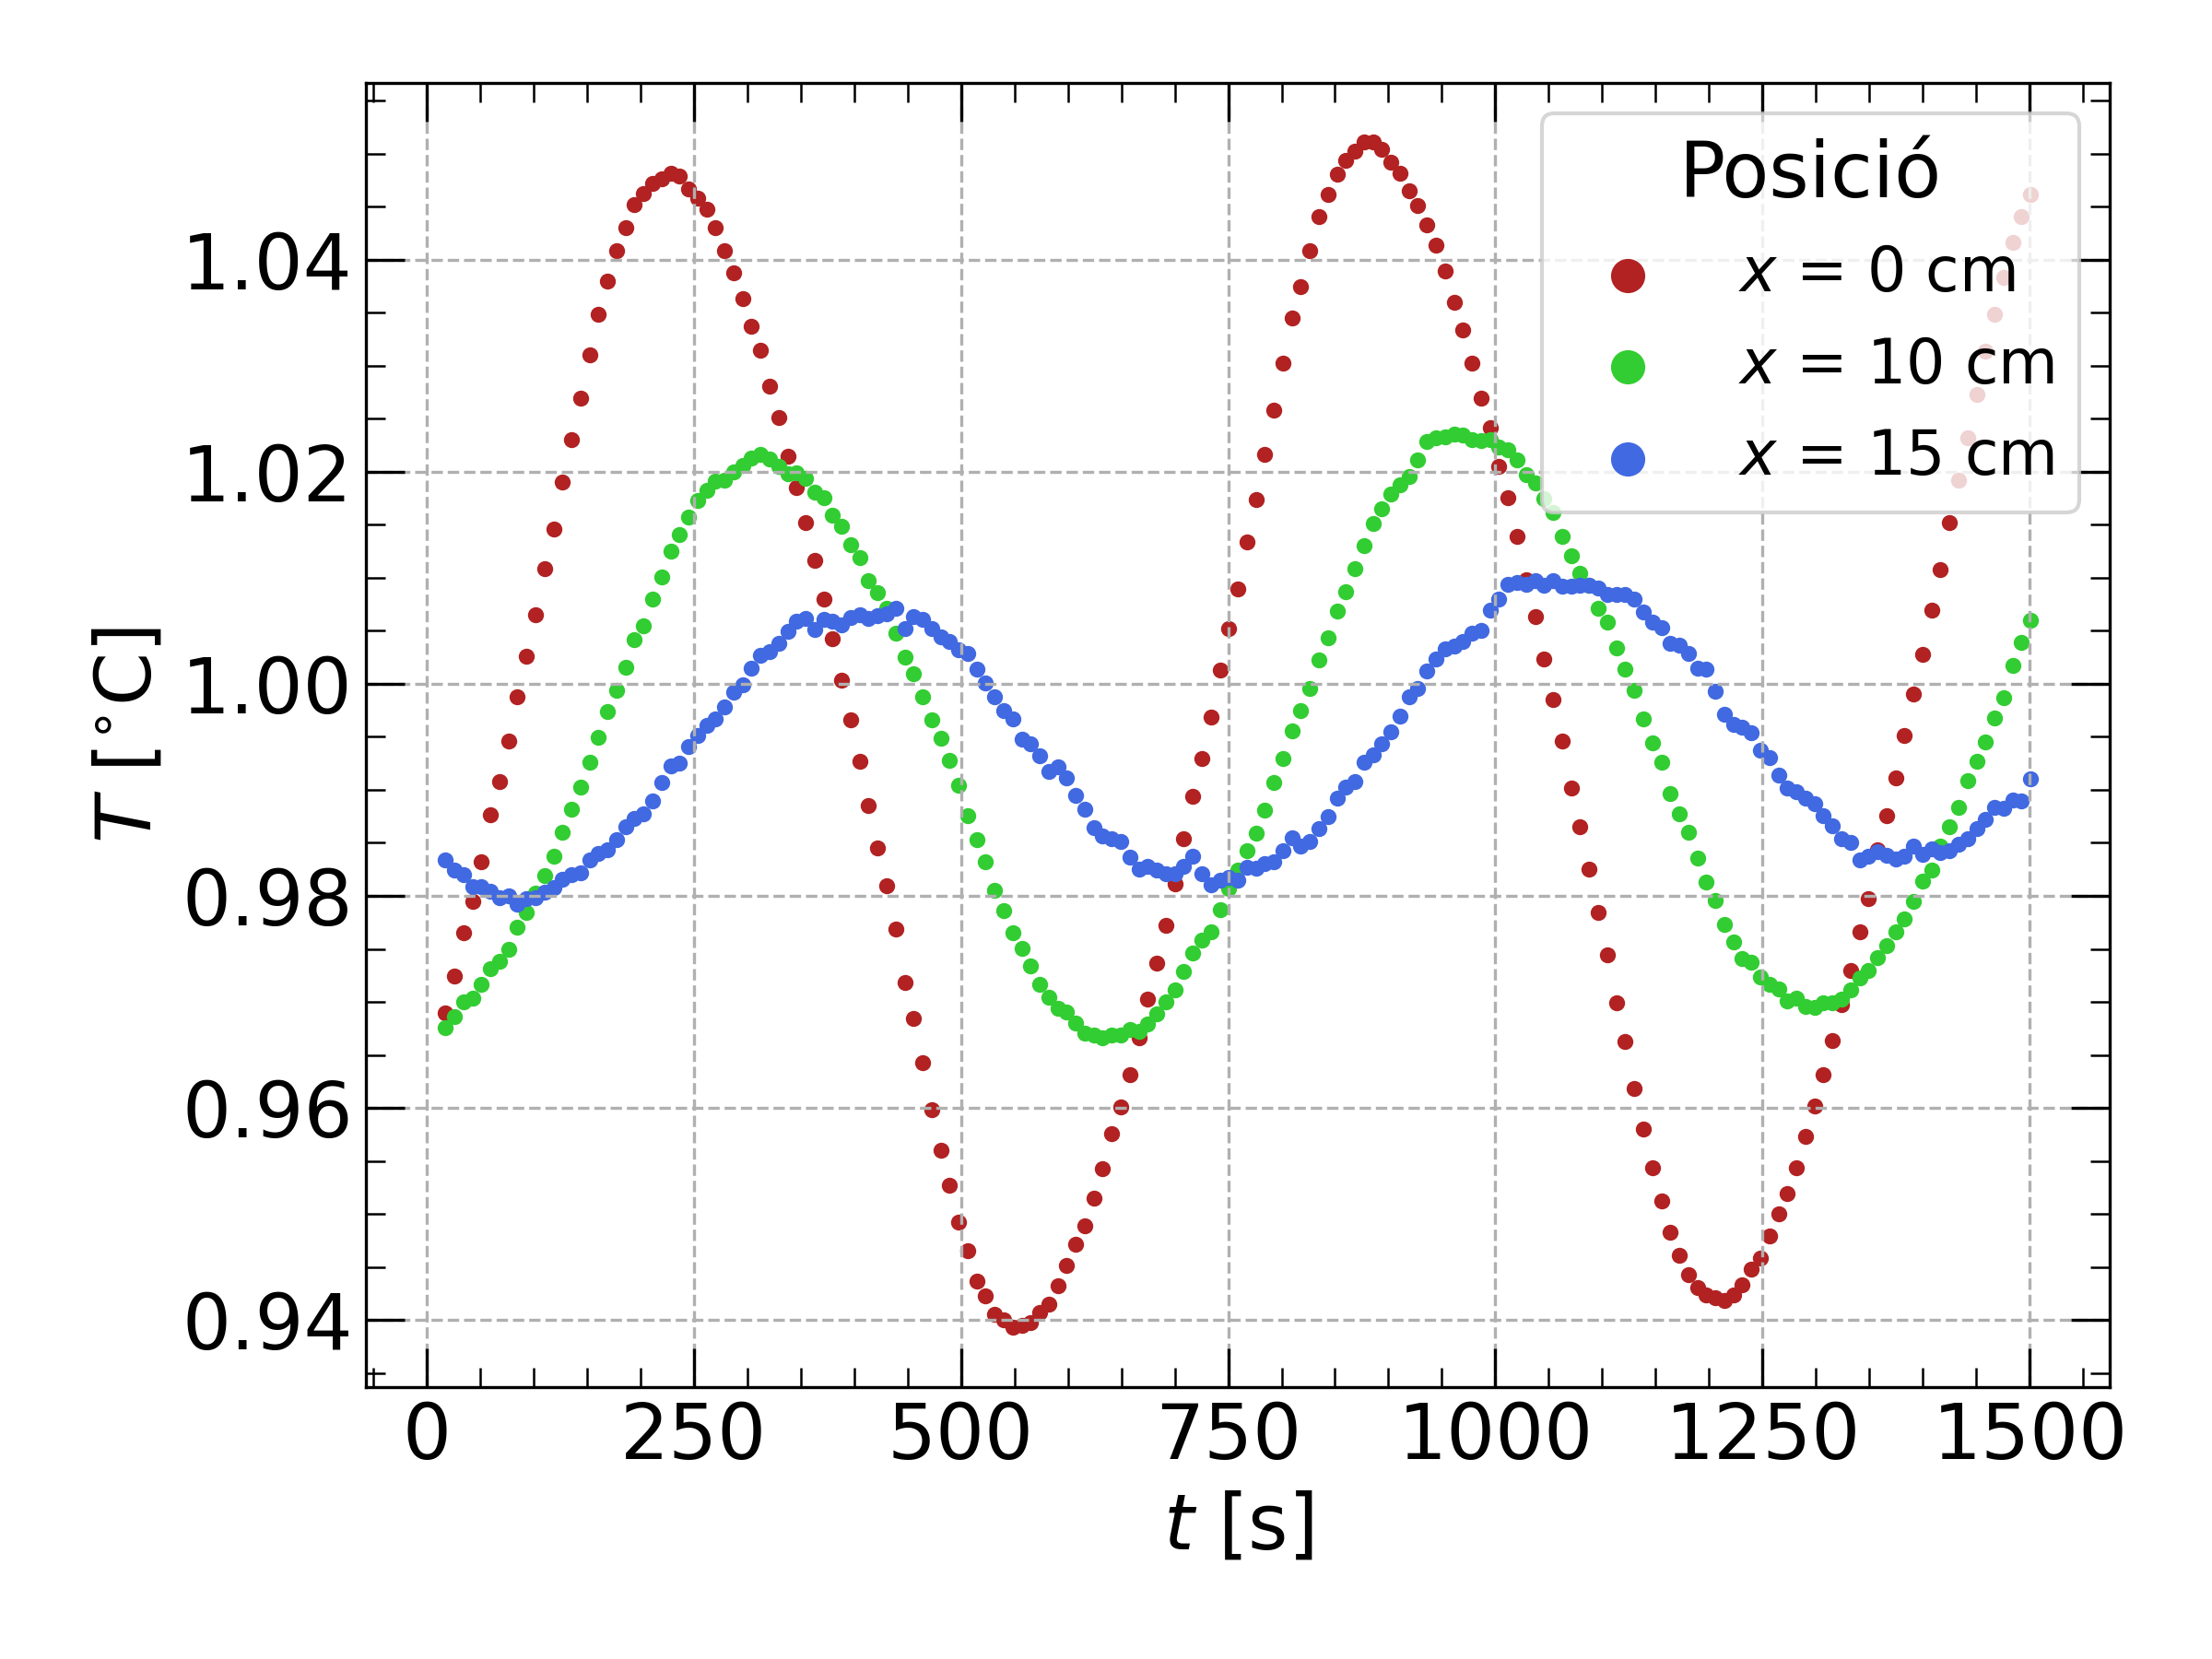
\includegraphics[width=1\linewidth]{../../graphs/practica_Ia/plots/petit_norm.png}
  \captionof{figure}{\footnotesize{Gràfica de $T$ en funció de $t$ normalitzada de la barra petita. Temperatures mesurades a una distància de \(0\,\text{cm}\) (vermell), \(10\,\text{cm}\) (verd) i \(20\,\text{cm}\) (blau) del punt de referència.}}
  \label{fig:T_vs_t_petita_norm}
\end{Figura}
Es pot obeservar com existeix desfasament entre dos punts diferents a cada barra, la ona tèrmica avança a mesura que augmenta la distància. A més, també es pot veure un comportament similar al que prediu l'Equació \eqref{desfasament}.\\\\
Per a determinar l'amplitud de la ona a cada punt per a cada barra escollim un punt màxim i un mínim consecutius i calculem la meitat de la diferència. Amb aquestes dades realitzem una mitjana i obtenim les amplituds que s'observen a la Taula \ref{tau:amplituds_mitjanes_gran} i a la Taula \ref{tau:amplituds_mitjanes_petita}.
\begin{Figura}
  \centering
  \captionof{table}{\footnotesize{Amplitud promig de la ona tèrmica sesgons la distància al punt de referència per a la barra gran.}}
  \begin{tabular}{c|c}
    $x_i$ ($\pm$0.1) [cm] & $\bar{a}_i$ ($\pm$0.001) [$^\circ$C]  \\ \hline
    0 & 2,963\\
    10 & 1,218\\
    15 & 0,802 
  \end{tabular}
  \label{tau:amplituds_mitjanes_gran}
\end{Figura} 
\begin{Figura}
  \centering
  \captionof{table}{\footnotesize{Amplitud promig de la ona tèrmica sesgons la distància al punt de referència per a la barra petita.}}
  \begin{tabular}{c|c}
    $x_i$ ($\pm$0.1) [cm] & $\bar{a}_i$ ($\pm$0.001) [$^\circ$C]  \\ \hline
    0 & 5,404\\
    10 & 2,273\\
    20 & 0,961  
  \end{tabular}
  \label{tau:amplituds_mitjanes_gran}
\end{Figura} 
Es pot observar com segueixen un comportament exponencial, similar al que hem vist a la Taula \ref{Tau:mitjanes}. Apliquem novament el mateix mètode amb les amplituds que amb les temperatures mitjanes i obtenim les regressions de la Figura \ref{fig:reg_lin_amplituds} i els valors dels pendents de la Taula \ref{tau:pendent_amplituds}.

\begin{Figura}
  \centering
  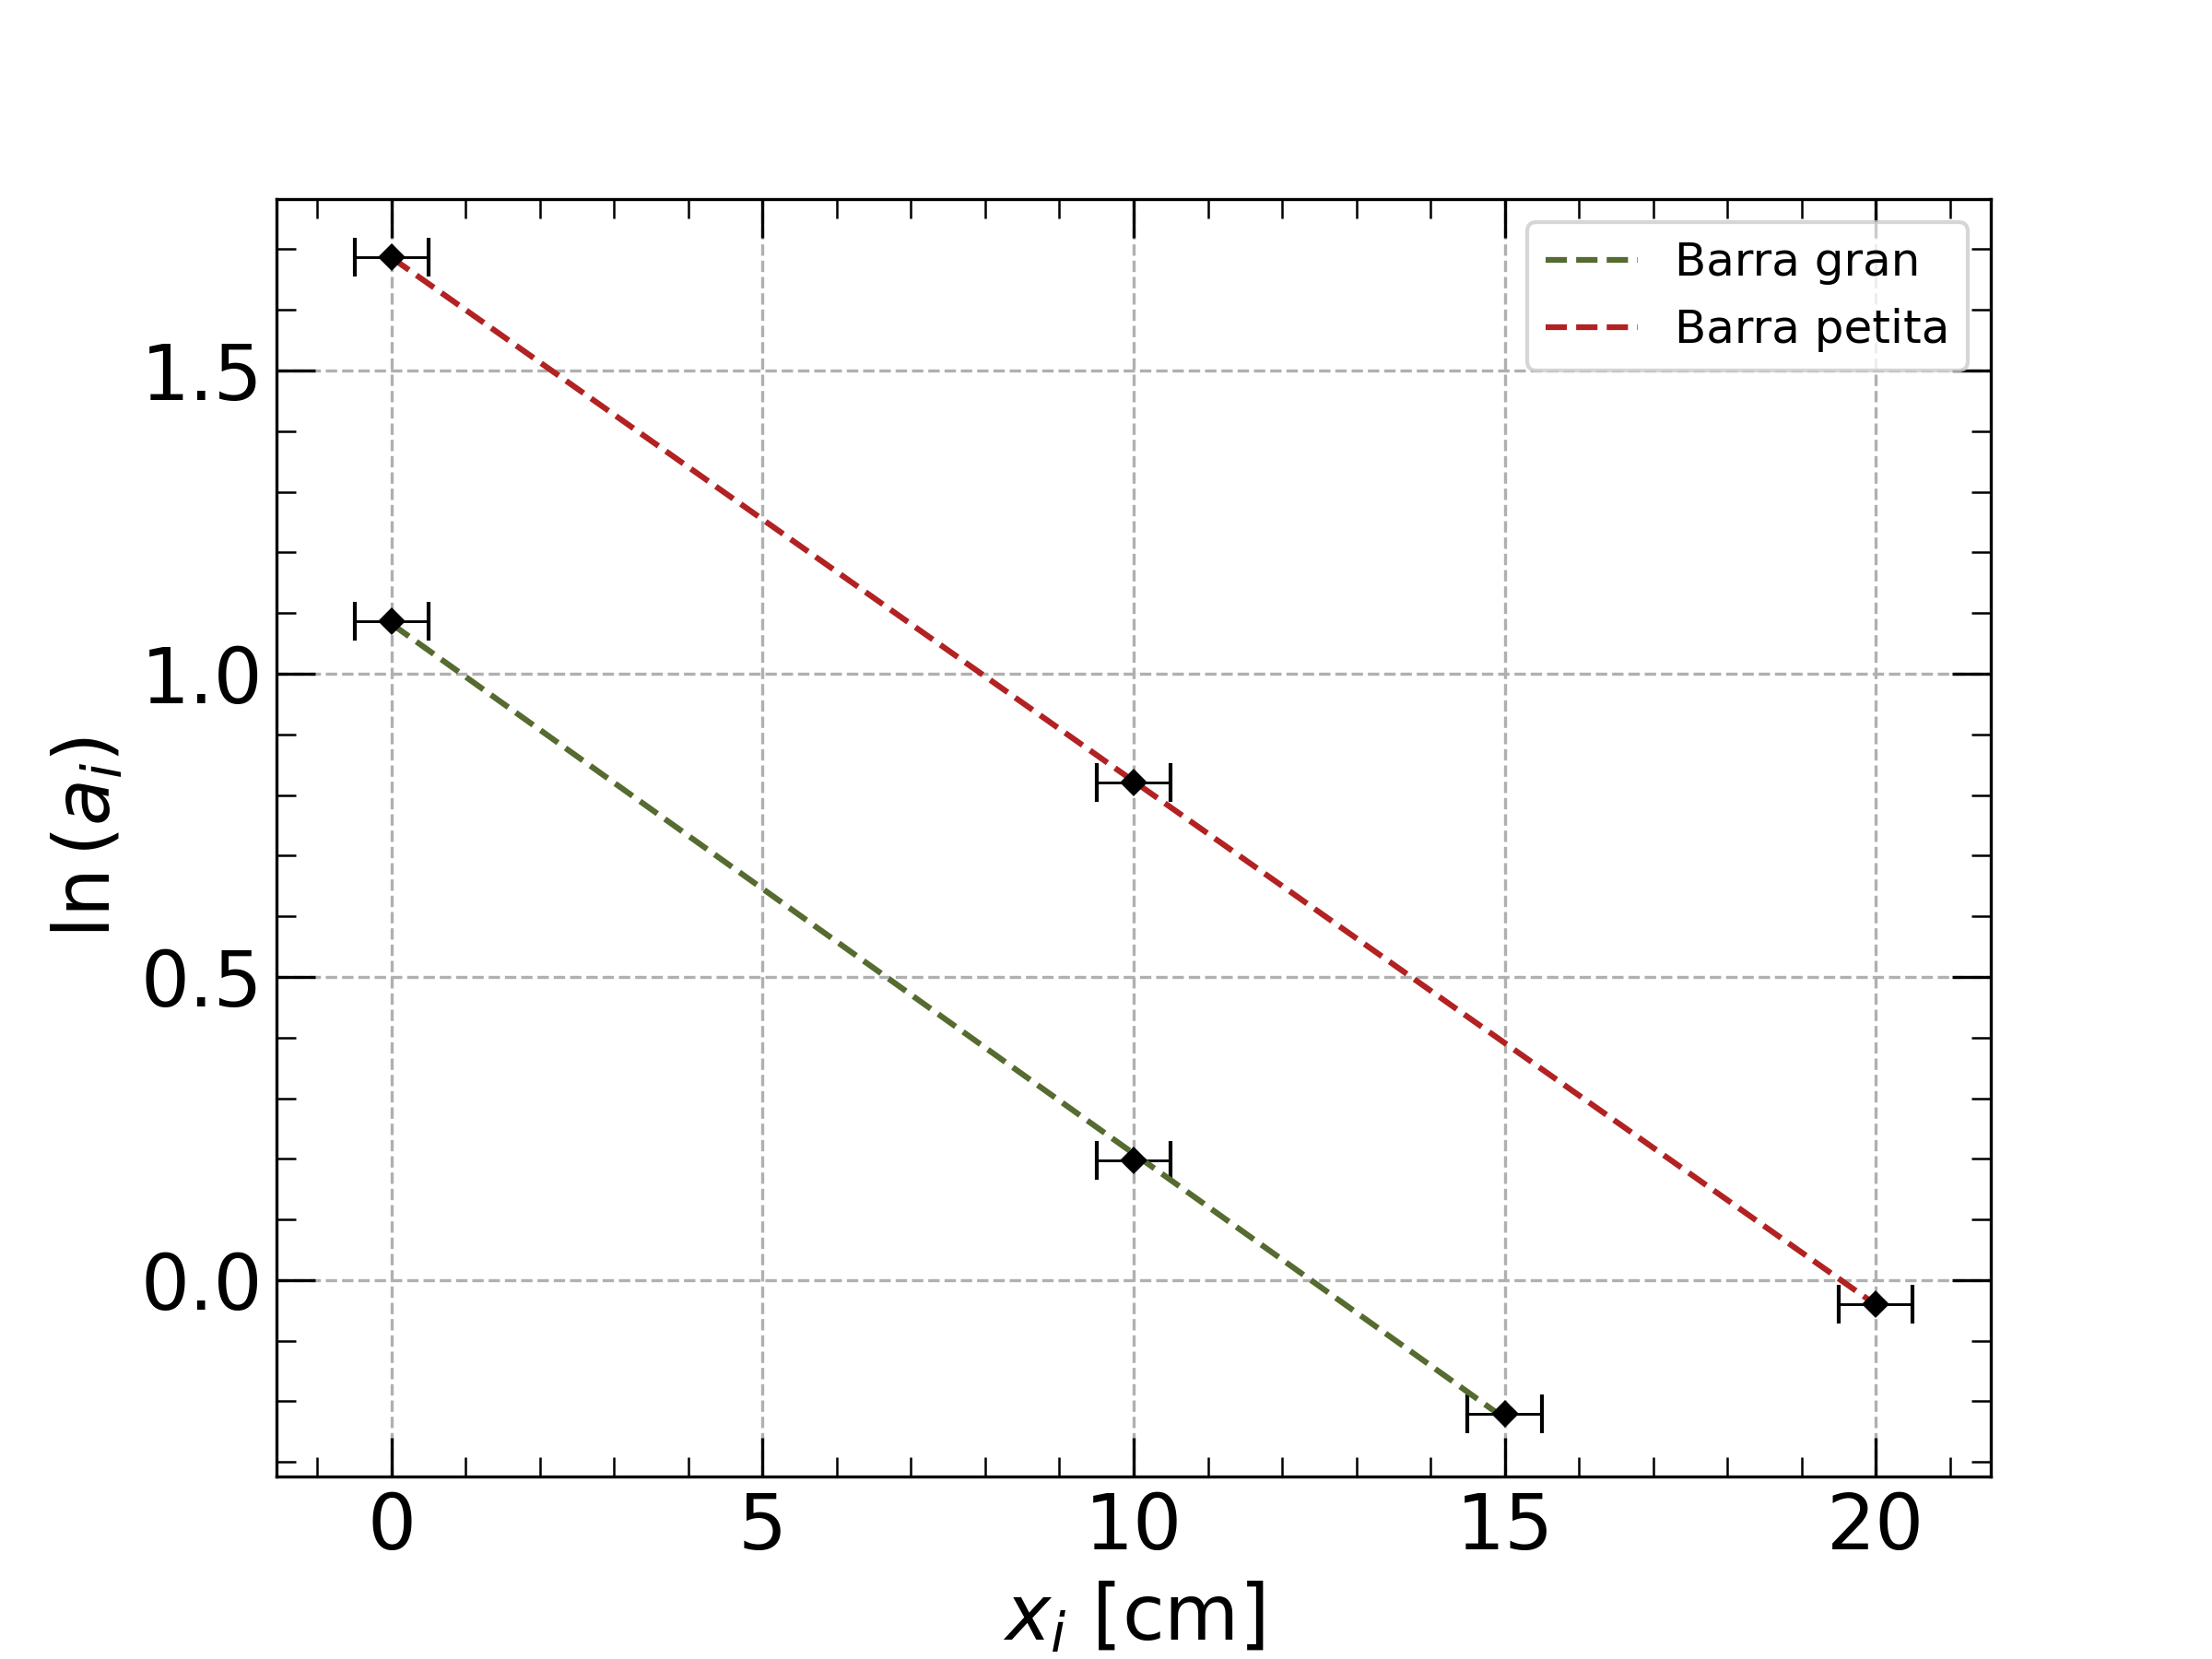
\includegraphics[width=1\linewidth]{../../graphs/practica_Ia/plots/reg_ampli.png}
  \captionof{figure}{\footnotesize{Regressió lineal del logaritme de les amplituds respecte a la posició. Coeficients de regressió obtinguts: $r^2$ = 0.999 tant per a la barra gran com per a la barar petita.}}
  \label{fig:reg_lin_amplituds}
\end{Figura}
\begin{Figura}
  \centering
  \captionof{table}{\footnotesize{Valors ajustats per a una regressió lineal, amb model $y = ax + b$, on $y$ és el logaritme de les amplituds i $x$ les posicions $x_i$.}}
  \begin{tabular}{c|c|c}
    Barra & $a$ ($\cdot 10^{-2}$) [cm$^{-1}$] & $b$ ($\cdot10^{-1}$) \\ \hline\hline
    gran & $-8,74\pm0,16$ & $10,82\pm0,14$\\
    petita & $-8,634\pm0,014$ & $16,862\pm0,018$ 
  \end{tabular}
  \label{tau:pendent_amplituds}
\end{Figura} 
Tenint en compte el comportament del desfasament i de les amplituds podem dir que les ones tèrmiques no són simètriques espaialment, decauen i pateixen un desfasament amb la distància.\\\\
Podem comprovar aquets resultats calculant el valor de $m$ a partir de l'Equació \ref{trobar_m}. Aplicant logaritme podem calcular $m$ per a qualsevol parell de posicions i qualsevol parell d'amplituds al mateix instant de temps. Escollim com a amplituds de referència les amplituds màximes trobades anteriorment. Calculem $m$ per a cada parell de màxims i fem la mitjana de tots per a cada barra. Aquest pas el repetim per a cada parell de posicions possible (veure Annex). Fent la mitjana de cada valor trobat acabem obtenint
\begin{equation*}
  \bar{m}_{\text{gran}} = (88,30\pm0,14)\cdot 10^{-3} \, \text{cm}^{-1}
\end{equation*}
per a la barra gran i
\begin{equation*}
  \bar{m}_{\text{petita}} = (86,343\pm0,037)\cdot 10^{-3} \, \text{cm}^{-1}
\end{equation*} 
per a la barra petita.\\\\
Comparant amb els pendent obtinguts a la Taula \ref{tau:pendent_amplituds} observem com, dins de la incertesa, els valors coincideixen.\\\\
Calculem ara el periode de les oscil·lacions. Per a fer-ho mesurem la distància entre els màxims trobats anteriorment, tot per a cada posició i cada barra. Trobem que, com calia esperar, aquests periodes d'oscil·lació són molt similars entre ells (veure Annex). Per tant, assumint que aquest periode és només un, donem el seu valor a partir de la mitjana de les dades trobades:
\begin{equation*}
  \bar{\tau} = (654,048\pm0,001) \, \text{s}
\end{equation*}
Sabent aquesta dada podem calcular el temps d'escalfament o de refredament mig senzillament dividint el periode a la meitat:
\begin{equation*}
  t_{\text{esc/ref}} = (325,024\pm0.001) \, \text{s}
\end{equation*}
Fent servir els màxims per a cada $x_i$ d'una mateixa barra podem calcular el desfasament entre dos punts. Tenint en compte l'Equació \eqref{increment_desfasament} podem calcular el valor de $h$ per a cada parell $x_i$. Fent la mitjana d'aquests valors i apliacnt-ho a cada barra trobem
\begin{equation*}
  \bar{h}_{\text{gran}} = (0,09\pm0,11) \, \text{cm}^{-1}
\end{equation*}
per a la barra gran i
\begin{equation*}
  \bar{h}_{\text{petita}} = (0,088\pm0,006) \, \text{cm}^{-1}
\end{equation*}
per a la barra petita.\\\\
Sabent tant els valors de $h$ i de $m$ per a cada barra podem calcular el valor de $\lambda$ segons l'equació \ref{valor_lambda}. Fem servir el valor de la conductivitat tèrmica de l'alumini trobat a la literatura a la secció anterior i com a radis fem servir
\begin{equation*}
  r_{\text{gran}} = (2,55\pm0.1)\, \text{cm}
\end{equation*}
\begin{equation*}
  r_{\text{petita}} = (1,5\pm0.1)\, \text{cm}
\end{equation*}
per ala barra gran i la barra petita, respectivament. Aleshores, calculem els valors de $\lambda$ i obtenim
\begin{equation*}
  \lambda_{\text{gran}} = (-0.08\pm0.72)\cdot 10^{-2} \, \text{W}/\text{Kcm}^{2}
\end{equation*}
\begin{equation*}
  \lambda_{\text{petita}} = (-0.04\pm0.19)\cdot 10^{-2} \, \text{W}/\text{K}\text{cm}^{2}
\end{equation*}
\section{Conclusions}
\end{multicols}
\section{Referencies}
http://hyperphysics.phy-astr.gsu.edu/hbasees/Tables/thrcn.html - d'on treiem les conductivitats termiques.
\end{document}
